\documentclass[11pt,a4paper]{article}

% --- Typography & Encodings ---
\usepackage[utf8]{inputenc}
\usepackage[T1]{fontenc}
\usepackage{lmodern}
\usepackage{microtype}
\usepackage{setspace}
\setstretch{1.15}

% --- Layout & Margins ---
\usepackage[margin=1in]{geometry}
\usepackage{titlesec}
\usepackage{fancyhdr}

% --- Mathematics & Science ---
\usepackage{amsmath}
\usepackage{amssymb}
\usepackage{chemformula}
\usepackage{siunitx}

% --- Graphics & Tables ---
\usepackage{graphicx}
\usepackage{booktabs}
\usepackage{tabularx}
\usepackage{makecell}
\usepackage{caption}
\usepackage{subcaption}
\captionsetup{font=small,labelfont=bf,labelsep=period}

% --- Citations & References ---
% Nature style citations (superscript without brackets in text)
\usepackage[super,sort&compress]{natbib}
\setcitestyle{super,comma}

% --- Hyperlinks & Colors ---
\usepackage{xcolor}
\definecolor{natureblue}{RGB}{0,70,140}
\usepackage[
    colorlinks=true,
    linkcolor=natureblue,
    citecolor=natureblue,
    urlcolor=natureblue,
    breaklinks=true
]{hyperref}

% --- Section Formatting (Nature Portfolio style) ---
\titleformat{\section}{\large\bfseries}{\thesection.}{0.5em}{}
\titleformat{\subsection}{\normalsize\bfseries}{\thesubsection}{0.5em}{}
\titleformat{\subsubsection}{\small\bfseries}{\thesubsubsection}{0.5em}{}

\pagestyle{fancy}
\fancyhf{}
\fancyhead[L]{\small\textit{npj Microgravity Review (In Preparation)}}
\fancyhead[R]{\small\thepage}
\renewcommand{\headrulewidth}{0.4pt}

\begin{document}

% --- Front Matter ---
\title{\textbf{\Large From Dust to Bio-Infrastructure: A Mechanistic Review of Sintered Regolith Ceramics for Lunar Biogenerative Life Support Systems}}

\author{
    \textbf{Richard J. Barker}$^{1,\dagger}$, \textbf{Laura E. Fackrell}$^{2}$, \textbf{Nicholas J. B. Brereton}$^{3}$, \textbf{Borja Barbero Barcenilla}$^{4}$, \textbf{Harmeet Multani}$^{1}$, \textbf{Harrison Coker}$^{5}$, and \textbf{Patrick Grove}$^{1}$
}

\date{
    \small
    $^{1}$NASA GeneLab / Open Science Data Repository (OSDR) Plant Analysis Working Group (AWG), Astromech Space Biology Lab\\
    $^{2}$NASA Jet Propulsion Laboratory / Planetary Protection \& Regolith Simulants Group\\
    $^{3}$School of Biology and Environmental Science, University College Dublin\\
    $^{4}$Department of Biochemistry and Biophysics, Texas A\&M University\\
    $^{5}$In-Situ Resource Utilization and Planetary Bioregenerative Systems Group\\[1ex]
    $^{\dagger}$Corresponding author: \texttt{dr.richard.barker@gmail.com}\\[2ex]
    \today
}

\maketitle

% --- Abstract & Keywords ---
\begin{abstract}
Sustaining a lunar presence requires closing Biogenerative Life Support Systems (BLSS), raising a central trade-study question: when does lunar regolith cultivation outperform Earth-imported hydroponics across mass, energy, crew time, and biological risk? Direct cultivation in raw regolith is constrained by nanophase metallic iron ($\mathrm{npFe}^0$), Fenton-mediated reactive oxygen species (ROS), silicate dangling bonds, and sharp mineral shards that arrest root growth. Under fractional lunar gravity ($1/6\,g$), reduced Bond numbers expand capillary rise sixfold, causing waterlogging, gas diffusivity collapse below the $D_p/D_o = 0.02$ percolation threshold, and hydraulic drift during root growth. Here, we evaluate four architectures across staged Artemis and MoonBase horizons: (1) conventional imported hydroponics, (2) direct raw or treated regolith, (3) a hydroponic--regolith hybrid with external bioleaching, and (4) sintered regolith ceramic bio-infrastructure. Thermal sintering ($>1050^\circ\mathrm{C}$) solid-solubilizes $\mathrm{npFe}^0$ into stable silicates, rounds grains, and constrains pore throats to $30\text{--}60\,\mu\mathrm{m}$, stabilizing matric potential ($-2.5$ to $-5.0\,\mathrm{kPa}$) and air-filled porosity ($>25\text{--}30\%$; $D_p/D_o \approx 0.086$). NASA BVAD-grounded Equivalent System Mass (ESM) modeling normalized to edible yield ($\mathrm{kg\ ESM/kg\ edible}$) shows conventional hydroponics or hybrids are optimal for short sorties, whereas sintered ceramics achieve parity with direct regolith within $9.4\,\mathrm{months}$ (nuclear) to $18\text{--}22\,\mathrm{months}$ (solar/RFC) and outperform conventional hydroponics beyond $20.5\,\mathrm{months}$ (6 crew; $10.9\,\mathrm{months}$ for 12 crew), driven by $>98.5\%$ water recovery and cyclic $500^\circ\mathrm{C}$ pyrolytic regeneration.
\end{abstract}

\vspace{0.5em}
\noindent\textbf{Keywords:} Lunar regolith, Biogenerative Life Support Systems, Hydroponics, ISRU, Porous ceramics, Reduced-gravity vadose physics, Equivalent System Mass.


\vspace{1em}
\hrule
\vspace{1.5em}

% --- Main Body Sections ---
\section{Introduction: The In-Situ Resource Utilization Imperative in Lunar Life Support}
\label{sec:introduction}

Establishing an enduring human presence on the lunar surface requires transitioning from open-loop, resupply-dependent life support architectures to closed-loop, regenerative Biogenerative Life Support Systems (BLSS)\cite{wheeler2017agriculture,paul2022plants,ming1989lunar}. Terrestrial logistics impose an unsustainable launch mass burden for multi-year surface missions, where crew metabolic requirements for water, oxygen, and fresh nutrition scale linearly with crew complement and mission duration\cite{hanford2004advanced,wheeler2003carbon}. Higher-plant bioregenerative architectures address this vulnerability by using photoautotrophic crop canopies to scrub atmospheric carbon dioxide ($\mathrm{CO}_2$), generate metabolic oxygen ($\mathrm{O}_2$), purify greywater via foliar transpiration, and produce fresh, nutrient-dense biomass\cite{wheeler2017agriculture,ming1989lunar,wheeler2003carbon}.

Historically, space mission trade studies evaluated two polarized edaphic approaches for planetary crop production: importing prefabricated hydroponic hardware from Earth, or cultivating crops directly in untreated, in-situ planetary regolith\cite{paul2022plants,ming1989lunar,wamelink2019crop}. Importing inert root-support matrices (such as mineral rockwool, polyurethane foams, or expanded clay) and prefabricated polymeric fluid channels from Earth imposes launch-mass penalties and recurring media-replacement logistics that constrain the deployable agricultural footprint during long-duration settlement\cite{ming1989lunar,hanford2004advanced,wamelink2019crop}. Recent International Space Station (ISS) flight demonstrations---notably NASA's Plant Water Management (PWM-5 and PWM-6) investigations---show that passive, open-channel capillary fluidics can eliminate disposable media and mechanical pumps in microgravity\cite{nasa_pwm,weislogel2026pwm,monje2026hydroponic}; however, importing 3D-printed polymeric troughs still incurs launch mass. Conversely, direct edaphic cultivation in raw lunar regolith---often termed ``direct regolith agriculture''---operates under the premise that lunar dust can serve as a functional analog to terrestrial soil once augmented with water and soluble fertilizers\cite{ming1989lunar,wamelink2019crop,atkin2024bioremediation}. Between these extremes lies a third hybrid architecture---combining reusable hydroponic channels with external regolith nutrient-recovery bioreactors---and a fourth in-situ manufacturing pathway: sintered regolith ceramic bio-infrastructure, which can fabricate both porous wicking matrices and PWM-style capillary channels directly from lunar dust.

However, botanical experiments utilizing returned Apollo specimens and high-fidelity lunar simulants demonstrate that raw regolith imposes severe physiological penalties\cite{paul2022plants,ming1989lunar,coker2026lunar}. Planetary-scale exposure to unattenuated solar wind protons, galactic cosmic rays, and hypervelocity micrometeorite comminution has produced a geochemically hostile matrix characterized by submicroscopic zero-valent metallic iron ($\mathrm{npFe}^0$), unweathered razor-sharp mineral edges, and volatile abiotic surface reactivity\cite{paul2022plants,ming1989lunar,hendrix2024reactivity,turci2015mechanistic}. Single-particle wettability determinations on returned Chang'e-5 samples also reveal pronounced intrinsic hydrophobicity across pristine lunar dust grains\cite{zhang2025wettability}. In parallel, the reduction of gravitational acceleration to one-sixth terrestrial gravity ($1/6\,g$) lowers the dimensionless Bond number sixfold, causing capillary retention forces to dominate over gravitational drainage\cite{ming1989lunar,steinberg2007fluid,jones1999microgravity,jones2012beyond}. As shown by reduced-gravity vadose-zone scaling\cite{jones2012beyond} and suborbital centrifuge flight experiments simulating lunar gravity ($1.76\,\mathrm{m/s}^2$), fluid menisci exhibit rounded curvatures and boundary film thickening, while hydrophobic surface dust impedes water infiltration and liquid-gas equilibration\cite{hasenstein2026assessing}. Mitigating root-zone hypoxia under fractional gravity requires coarse, well-aerated aggregates ($0.5\text{--}2.0\,\mathrm{mm}$)\cite{stout2001evidence,hasenstein2026assessing,jones2012beyond}; however, core stratigraphy from Apollo and Chang'e-5 drill cores confirms that such millimeter-scale fractions dominate only at depths of several meters\cite{mckay1991lunar,zhao2023variations}, imposing substantial mechanical excavation and sifting burdens on early human outposts.

To overcome both the launch-mass penalty of imported hardware and the biological toxicity of raw regolith, life-support engineering is converging toward an in-situ bio-infrastructure paradigm\cite{ming1989lunar,taylor2005microwave,fateri2019solar}. Rather than framing hydroponic systems and regolith-based agriculture as mutually exclusive alternatives, this review synthesizes a phased, modular architecture for lunar BLSS: early expeditionary missions ($2\text{ weeks}\text{--}6\text{ months}$) rely on closed-loop, soil-less hydroponic and passive capillary modules—benchmarked against terrestrial closed-loop urban CEA systems (e.g., Lufa Farms) and flight-validated in NASA's Plant Water Management (PWM-5/6, PSI-187) experiments\cite{weislogel2026pwm,hatch2022pwm,pwm2020ntrs}—whereas long-duration settlements ($1\text{ year}\text{--}\text{permanent}$) progressively integrate ISRU thermal consolidation to transform sieved regolith fines into engineered porous ceramics\cite{ming1989lunar,taylor2005microwave,xi2026multiphysics}. High-temperature sintering passivates reactive geochemical interfaces, rounds abrasive grain morphology, and enables the precision fabrication of hydroponic troughs, multiphase fluid-delivery wicks, LECA-like expanded clay aggregate replacements, and mycoponic scaffolds\cite{ming1989lunar,xi2026multiphysics,goulas2017process}. Coupled with open-science multi-omics baselines from the NASA Open Science Data Repository (OSDR; e.g., \texttt{OSD-267}, \texttt{OSD-269}, \texttt{OSD-655})\cite{gebre2025nasa}, this review analyzes the physicochemical, toxicological, fluid-mechanical, and systems-engineering principles that govern the transition from raw regolith farming to sintered ceramic bio-infrastructure for sustained lunar and Martian ($0.38\,g$) settlement.

\section{Physicochemical and Toxicological Interfaces of Pristine Lunar Regolith}
\label{sec:toxicology}

\subsection{Nanophase Iron and Abiotic Reactive Oxygen Species Generation}
\label{subsec:npfe_ros}

The Moon's hyper-vacuum environment and absence of a global dipolar magnetosphere expose surface minerals to unattenuated space weathering\cite{paul2022plants,ming1989lunar,hendrix2024reactivity,turci2015mechanistic}. Solar wind proton bombardment reduces ferrous silicates, while episodic micrometeorite impacts induce localized shock melting and vapor-phase condensation\cite{ming1989lunar,liu2013microwave}. These energetic processes generate nanophase metallic iron ($\mathrm{npFe}^0$), consisting of zero-valent iron blebs ($1\text{--}100\,\mathrm{nm}$ in diameter) embedded within mineral rims and dispersed throughout the amorphous silicate matrices of agglutinitic glasses\cite{paul2022plants,ming1989lunar,krejci2026lunar}.

When pristine regolith or reduced lunar simulants contact oxygenated aqueous solutions within a pressurized habitat, these surface-accessible metallic blebs trigger abiotic oxidation cascades\cite{ming1989lunar,hendrix2024reactivity,turci2015mechanistic}. Solvated divalent ferrous ions ($\mathrm{Fe}^{2+}$) dissolve from mineral interfaces in the presence of dissolved oxygen, initiating modified Fenton-like catalytic cycles\cite{ming1989lunar,hendrix2024reactivity,turci2015mechanistic}:
\begin{equation}
    \mathrm{Fe}^0 + \mathrm{O}_2 + 2\mathrm{H}^+ \longrightarrow \mathrm{Fe}^{2+} + \mathrm{H}_2\mathrm{O}_2
    \label{eq:fe0_dissolution}
\end{equation}
Subsequent electron transfer between the released ferrous iron and ambient oxidants drives the generation of hydroxyl free radicals ($\cdot\mathrm{OH}$) and superoxide radical anions ($\mathrm{O}_2^{\cdot-}$):
\begin{align}
    \mathrm{Fe}^{2+} + \mathrm{H}_2\mathrm{O}_2 &\longrightarrow \mathrm{Fe}^{3+} + \cdot\mathrm{OH} + \mathrm{OH}^- \label{eq:fenton_reaction} \\
    \mathrm{Fe}^{2+} + \mathrm{O}_2 &\longleftrightarrow \mathrm{Fe}^{3+} + \mathrm{O}_2^{\cdot-} \label{eq:superoxide_reaction}
\end{align}

Electron paramagnetic resonance (EPR) spectroscopy with spin-trapping adducts, alongside chemical terephthalate hydroxylation assays, confirms that reduced lunar materials generate hydroxyl radical concentrations 5-fold to 100-fold higher than unreduced terrestrial basaltic analogs\cite{hendrix2024reactivity,turci2015mechanistic,wallace2022assessment}. Furthermore, mechanical impact crushing on the airless lunar surface cleaves covalent bonds in silicates, plagioclase, and pyroxenes without atmospheric passivating agents, leaving surface dangling bonds such as broken silicon radicals ($\equiv\!\mathrm{Si}\cdot$) and silicon-peroxyl radicals ($\equiv\!\mathrm{Si}-\mathrm{O}\cdot$)\cite{turci2015mechanistic,hendrix2019measurement}. Upon hydration, these radicals homolytically split water molecules, generating sustained bursts of oxidizing species\cite{hendrix2019measurement,sperl2017influence}. Direct contact with this abiotic interface subjects plant root cell membranes to rapid lipid peroxidation, disrupting transmembrane electrochemical gradients, destroying transport proteins, and inducing root apical growth arrest\cite{ming1989lunar,turci2015mechanistic}.

\subsection{Transcriptomic Reprogramming, Genomic Lesions, and Morphological Impedance}
\label{subsec:transcriptomics_genomics}

The biological consequences of these reactive interfaces were demonstrated empirically by Paul et al.\cite{paul2022plants} using authentic lunar soils returned by Apollo 11, 12, and 17. Seeds of \textit{Arabidopsis thaliana} germinated uniformly across Apollo regolith samples and volcanic controls; however, post-germination ontogeny diverged sharply\cite{paul2022plants}. Seedlings cultivated directly in Apollo regoliths exhibited severe stress phenotypes, including arrested primary root elongation, stunted rosette expansion, retarded leaf development, and dark purple pigmentation driven by anthocyanin hyperaccumulation\cite{paul2022plants}.

High-throughput RNA sequencing revealed that plants grown in raw lunar regolith execute a systemic transcriptomic reprogramming, shifting metabolic resources from vegetative biomass accumulation to protective defense cascades\cite{paul2022plants,krejci2026lunar}. Differentially expressed genes are dominated by pathways associated with heavy metal toxicity, osmotic shock, and oxidative burst defense\cite{paul2022plants,krejci2026lunar}. Plants significantly upregulate transcripts encoding glutathione S-transferases (GSTs), class III secretory cell-wall peroxidases, heat shock transcription factors, and antioxidant enzymes\cite{paul2022plants,krejci2026lunar}. Concurrently, signaling cascades mediated by jasmonic acid (JA) and abscisic acid (ABA) are chronically induced, repressing cell-wall loosening and cellular expansion\cite{paul2022plants,ming1989lunar}. The magnitude of transcriptomic stress correlates positively with regolith maturity, quantified by the ferromagnetic resonance (FMR) maturity index ($I_s/\mathrm{FeO}$)\cite{paul2022plants,morris1976surface}. Mature regoliths (e.g., Apollo 11 sample 10084 and Apollo 17 sample 70051), possessing high agglutinitic glass and $\mathrm{npFe}^0$ contents, trigger significantly more intense stress responses than immature sub-surface samples (e.g., Apollo 12 sample 12070)\cite{paul2022plants}.

Beyond immediate physiological stress, continuous root exposure to raw regolith compromises long-term genomic stability\cite{barbero2024telomere,shippen2019telomere}. Multi-generational cultivation experiments utilizing regolith simulants demonstrate progressive accumulation of 8-oxoguanine (8-oxoG) DNA lesions induced by oxidative stress\cite{barbero2024telomere}. Because chromosomal telomeres contain repetitive guanine-rich motifs, they act as primary targets for oxidative damage\cite{barbero2024telomere,min2023protection}. In regolith simulant environments, telomerase catalytic activity becomes uncoupled from telomere length maintenance, culminating in accelerated telomere shortening, genome instability, and loss of multi-generational fitness\cite{ming1989lunar,barbero2024telomere}.

These biochemical challenges are compounded by particle morphometry\cite{paul2022plants,ming1989lunar,fackrell2024mechanical}. Lacking atmospheric tumbling or aqueous rounding regimes, lunar particles retain razor-sharp edges with extreme aspect ratios\cite{paul2022plants,ming1989lunar,fackrell2024mechanical}. As expanding root tips penetrate these interlocking angular grains, the abrasive surfaces micro-shear the root cap, strip mucilage-secreting border cells, and tear epidermal tissues\cite{ming1989lunar,hendrix2024reactivity}. Plants must continuously expend metabolic energy repairing damaged epidermal barriers, resulting in a systemic physiological penalty that curtails edible crop yields\cite{ming1989lunar,fackrell2024mechanical}.

\begin{figure}[t!]
    \centering
    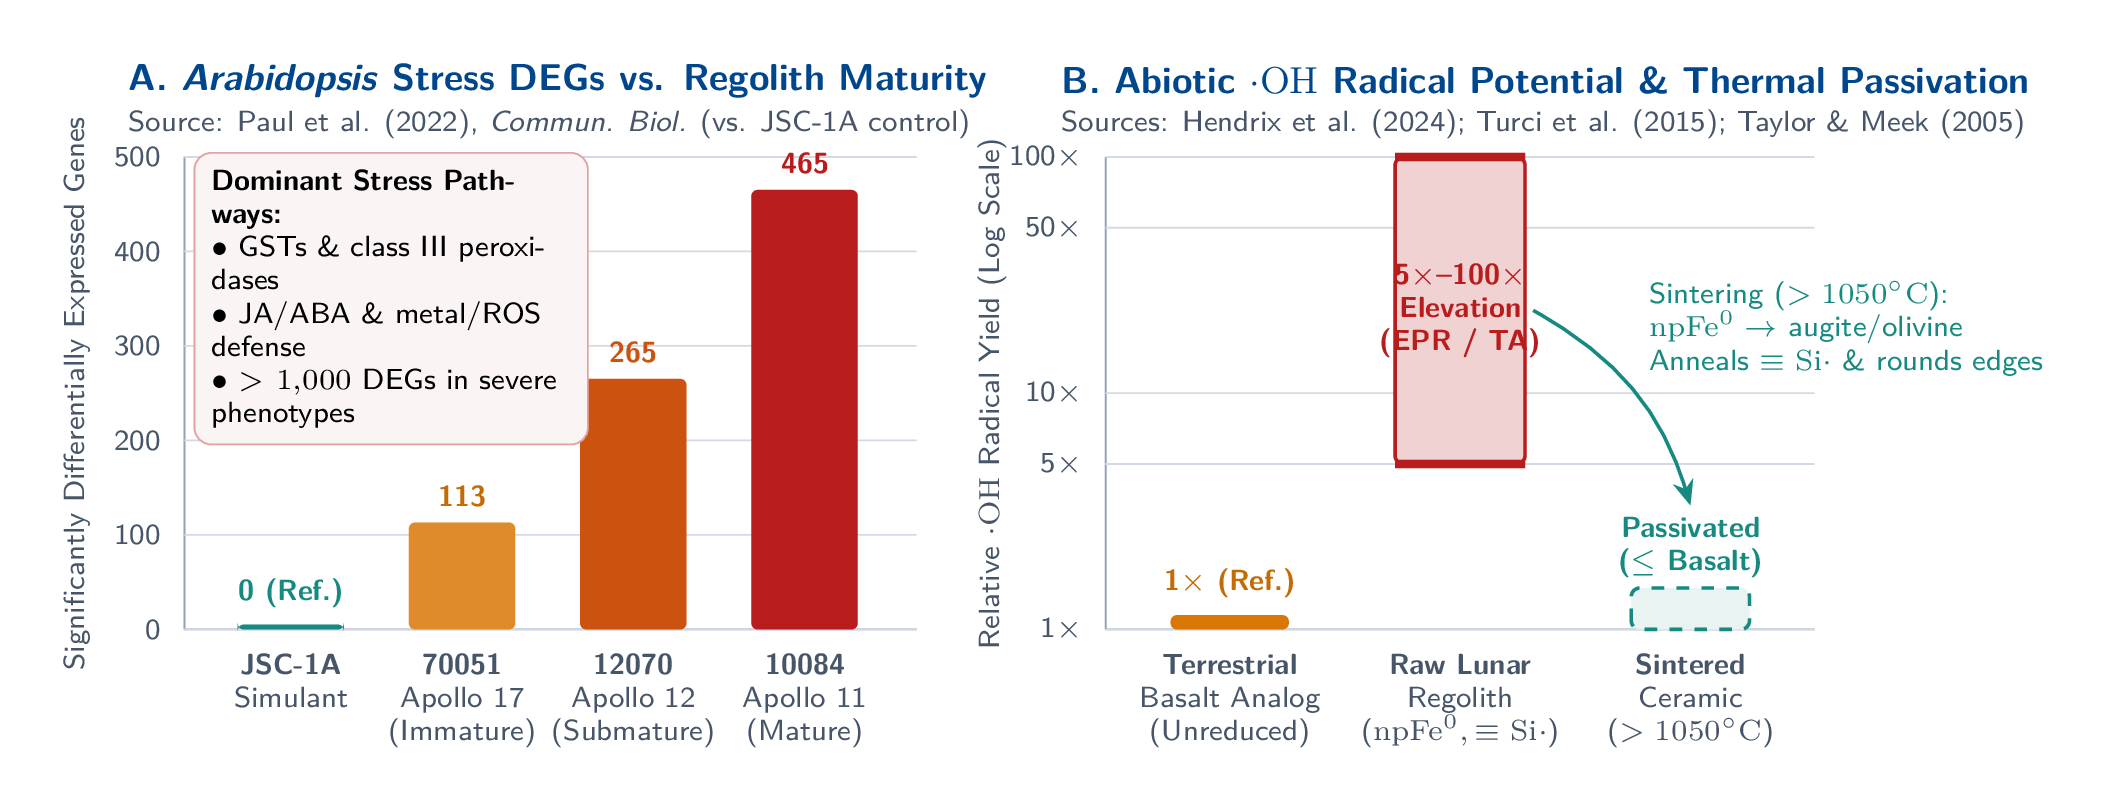
\includegraphics[width=0.92\textwidth]{figures/fig1_toxicity_passivation.png}
    \caption{\textbf{Physicochemical and toxicological interfaces of raw versus sintered lunar regolith.} (\textbf{a}) Raw lunar regolith contains reactive nanophase metallic iron ($\mathrm{npFe}^0$), broken silicate dangling bonds, and razor-sharp mineral shards that generate chronic oxidative stress via modified Fenton reactions ($\mathrm{Fe}^0 \to \mathrm{Fe}^{2+} \to \cdot\mathrm{OH}, \mathrm{O}_2^{\cdot-}$), damaging plant root membranes and inducing 8-oxoG genomic lesions. (\textbf{b}) Thermal sintering above $1050^\circ\mathrm{C}$ passivates these hazards by oxidizing $\mathrm{npFe}^0$ into stable augite and olivine crystal matrices, rounding abrasive grain boundaries, and restoring plant transcriptomic homeostasis.}
    \label{fig:toxicity_passivation}
\end{figure}

\begin{table}[t!]
\small
\centering
\caption{\textbf{Comparative physicochemical, toxicological, and agronomic properties of raw lunar regolith versus sintered regolith ceramics.}}
\label{tab:toxicity_comparison}
\begin{tabularx}{\textwidth}{lXX}
\toprule
\textbf{Parameter / Property} & \textbf{Raw Lunar Regolith (Direct Cultivation)} & \textbf{Sintered Regolith Ceramic (Engineered Substrate)} \\
\midrule
Nanophase Metallic Iron ($\mathrm{npFe}^0$) & Surface-accessible blebs across grain rims ($1\text{--}100\,\mathrm{nm}$)\cite{paul2022plants,ming1989lunar,krejci2026lunar} & Oxidized and incorporated into stable crystalline silicates\cite{ming1989lunar,taylor2005microwave} \\
\addlinespace
Aqueous ROS Generation Potential & High; sustained $\cdot\mathrm{OH}$ and $\mathrm{O}_2^{\cdot-}$ generation via Fenton pathways\cite{paul2022plants,hendrix2024reactivity,turci2015mechanistic} & Negligible; passivated, hydrothermally inert interface\cite{ming1989lunar,turci2015mechanistic,sperl2017influence} \\
\addlinespace
Grain / Pore Morphometry & Highly angular, sharp, micro-shearing shards\cite{ming1989lunar,hendrix2024reactivity,fackrell2024mechanical} & Rounded, smooth, consolidated neck boundaries\cite{ming1989lunar,xi2026multiphysics,goulas2017process} \\
\addlinespace
Plant Transcriptomic Profile & Chronic upregulation of GSTs, peroxidases, JA, and ABA stress pathways\cite{paul2022plants,krejci2026lunar} & Homeostatic baseline; standard vegetative and reproductive allocation\cite{paul2022plants,ming1989lunar} \\
\addlinespace
Chromosomal \& Telomeric Integrity & Elevated 8-oxoG lesions, accelerated telomere erosion, fitness decline\cite{barbero2024telomere,shippen2019telomere,min2023protection} & Protected genome; absence of mineral-derived radical stress\cite{ming1989lunar,barbero2024telomere} \\
\addlinespace
Interfacial Contact Angle & Initially hydrophobic; prone to liquid beading and bypass channeling\cite{paul2022plants,steinberg2007fluid} & Tailored hydrophilic wettability; continuous capillary wicking\cite{ming1989lunar,heinse2007porous} \\
\addlinespace
Aqueous Solution Chemistry & Uncontrolled dissolution; alkaline spikes ($\mathrm{pH}\;9.0\text{--}11.0$), P-fixation\cite{ming1989lunar,hendrix2024reactivity,wamelink2024struvite} & Stable $\mathrm{pH}$ control ($\mathrm{pH}\;5.8\text{--}6.2$); predictable nutrient stoichiometry\cite{ming1989lunar} \\
\bottomrule
\end{tabularx}
\end{table}

\section{Materials Science and In-Situ Manufacturing Modalities for Bio-Infrastructure}
\label{sec:manufacturing}

\subsection{Solid-State Sintering and Surface Passivation Mechanisms}
\label{subsec:sintering_mechanisms}

Thermal sintering between $1050^\circ\mathrm{C}$ and $1250^\circ\mathrm{C}$ transforms loose, biologically reactive lunar regolith into chemically passivated, structurally coherent porous ceramics\cite{ming1989lunar,xi2026multiphysics,sperl2017influence}. Within this thermal envelope, consolidation initiates via solid-state diffusion and localized liquid-phase sintering\cite{ming1989lunar}. Agglutinitic impact glasses and low-melting-point pyroxenes soften and undergo viscous flow, wetting adjacent refractory mineral grains---primarily anorthitic plagioclase---and creating consolidated neck boundaries across particle contact zones\cite{ming1989lunar,xi2026multiphysics}.

This thermal restructuring passivates the biological hazards of pristine regolith through two coordinated transformations\cite{ming1989lunar}:
\begin{enumerate}
    \item \textbf{Geochemical Passivation of Metallic Iron:} Thermal processing in controlled atmospheres oxidizes the submicroscopic zero-valent iron blebs\cite{ming1989lunar}. Above $1000^\circ\mathrm{C}$, metallic $\mathrm{npFe}^0$ oxidizes and diffuses into softening aluminosilicate melts, solid-solubilizing into thermodynamically stable crystalline phases, principally clinopyroxenes (such as augite, $(\mathrm{Ca, Mg, Fe})\mathrm{SiO}_3$) and olivines ($(\mathrm{Mg, Fe})_2\mathrm{SiO}_4$)\cite{ming1989lunar,schoonen2020hydroxyl,meek1993mechanical}. Once immobilized within silicate crystal lattices, iron ions can no longer undergo redox cycling in aqueous solution, quenching Fenton-mediated free radical cascades\cite{paul2022plants,ming1989lunar}.
    \item \textbf{Morphological Rounding and Quenching of Dangling Bonds:} Viscous sintering smooths razor-sharp mineral edges\cite{ming1989lunar}. High interfacial surface energies drive atomic mass transfer from convex surfaces into concave neck junctions, transforming jagged grain edges into rounded, smooth pore walls\cite{ming1989lunar}. This atomic rearrangement quenches reactive surface dangling bonds ($\equiv\!\mathrm{Si}\cdot$, $\equiv\!\mathrm{Si}-\mathrm{O}\cdot$) and eliminates the micro-shearing geometries that damage root apical meristems\cite{ming1989lunar,turci2015mechanistic,xi2026multiphysics}. The resulting ceramic matrix is non-abrasive, chemically passivated, and biocompatible with root systems and beneficial rhizosphere microflora\cite{ming1989lunar,hendrix2024reactivity}.
\end{enumerate}

\subsection{Advanced Manufacturing Modalities}
\label{subsec:modalities}

Fabricating functional bio-infrastructure from raw regolith requires thermal consolidation techniques matched to lunar surface environmental and power constraints\cite{ming1989lunar,fateri2019solar,goulas2017process}. Three primary modalities have been validated through terrestrial laboratory testing and planetary analog campaigns (Figure~\ref{fig:sintering_radar} and Table~\ref{tab:manufacturing_modalities}):

\subsubsection{Microwave Sintering}
Microwave processing at frequencies of $2.45\,\mathrm{GHz}$ and $5.8\,\mathrm{GHz}$ provides rapid, volumetric dielectric heating of the regolith bulk\cite{taylor2005microwave,xi2026multiphysics,lim2019numerical}. The absorbed electromagnetic power per unit volume ($P_v$, $\mathrm{W/m}^3$) is governed by:
\begin{equation}
    P_v = 2\pi f \varepsilon_0 \varepsilon'' |E|^2
    \label{eq:microwave_heating}
\end{equation}
where $f$ is the electromagnetic frequency ($\mathrm{Hz}$), $\varepsilon_0$ is the permittivity of free space ($8.854 \times 10^{-12}\,\mathrm{F/m}$), $\varepsilon''$ is the relative dielectric loss factor of the regolith, and $E$ is the root-mean-square electric field strength ($\mathrm{V/m}$)\cite{taylor2005microwave,xi2026multiphysics,lim2019numerical}.

Lunar regolith couples strongly with microwave radiation because its dielectric loss tangent ($\tan\delta = \varepsilon''/\varepsilon'$) is elevated by the presence of distributed $\mathrm{npFe}^0$, ilmenite ($\mathrm{FeTiO}_3$), and structural defects in agglutinitic glasses\cite{taylor2005microwave,chen2024measurement}. This strong coupling allows pristine regolith to heat volumetrically from within, reaching sintering temperatures with lower specific energy consumption ($\sim 1.2\,\mathrm{kWh/kg}$) than surface heating methods\cite{taylor2005microwave,lim2019numerical}. However, multiphysics modeling coupling electromagnetic radiation, heat transfer, and mechanical stress shows that non-uniform field distributions create steep thermal gradients\cite{xi2026multiphysics}. To avoid tensile stress exceeding the rupture modulus of sintered regolith ceramics, cooling rates must be strictly constrained to $<15^\circ\mathrm{C/min}$, preventing thermal microcracking and loss of fluid containment integrity\cite{xi2026multiphysics}.

\subsubsection{Concentrated Solar Sintering}
Concentrated solar sintering uses parabolic mirrors, heliostats, or Fresnel concentrators to direct ambient solar irradiance ($I_0 \approx 1361\,\mathrm{W/m}^2$) directly onto the regolith bed\cite{ming1989lunar,fateri2019solar}. As demonstrated by projects such as the European Space Agency's RegoLight initiative, solar concentrators can achieve focal temperatures above $1400^\circ\mathrm{C}$ in a vacuum without consuming habitat electrical power\cite{ming1989lunar,fateri2019solar,meurisse2018regolight,meurisse2018solar}.

Because concentrated radiative flux deposits energy purely at the material boundary, inward heat transfer relies on thermal conduction, which is constrained by the extremely low thermal conductivity of porous regolith in vacuum\cite{xi2026multiphysics,lim2019numerical}. Consequently, effective thermal penetration depth is restricted to $<10\,\mathrm{mm}$ per pass\cite{xi2026multiphysics}. Concentrated solar sintering is therefore executed via Additive Layer Manufacturing (ALM), fusing successive thin powder layers to build large structural elements such as heavy-walled hydroponic troughs, drainage channels, and bulk radiation shielding during the 14-day lunar day\cite{ming1989lunar,meurisse2018regolight,fateri2018additive}.

\subsubsection{Selective Laser Melting (SLM)}
Selective Laser Melting (SLM) and Selective Laser Sintering (SLS) direct a continuous-wave laser beam (typically near-infrared, $\lambda = 1064\,\mathrm{nm}$) across a pre-spread powder bed of classified regolith\cite{ming1989lunar,goulas2017process,goulas2024selective}. The focused beam generates a localized melt pool that completely liquefies and vitrifies the silicate minerals, offering dimensional feature tolerances below $50\text{--}100\,\mu\mathrm{m}$\cite{xi2026multiphysics,goulas2017process}.

While SLM requires higher specific electrical energy ($\sim 3.5\,\mathrm{kWh/kg}$) and exhibits lower volumetric build throughput than bulk microwave or solar sintering, its precision makes it indispensable for fabricating intricate fluid-handling bio-infrastructure\cite{ming1989lunar,goulas2017process}. These include two-phase aeration nozzles, non-clogging porous irrigation emitters, internal capillary manifolds, and passive open-wedge hydroponic troughs and bubble diverters modeled on flight-proven capillary fluidic geometries\cite{ming1989lunar,goulas2017process,balla2021selective,weislogel2026pwm}.

\begin{figure}[t!]
    \centering
    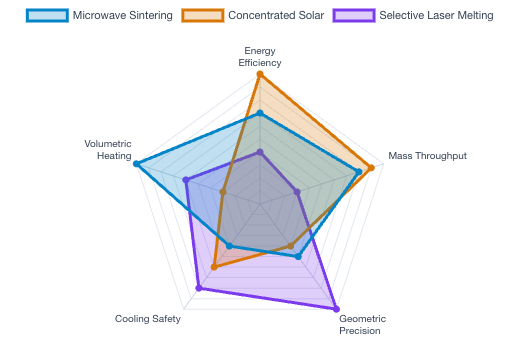
\includegraphics[width=0.75\textwidth]{figures/fig2_sintering_radar.png}
    \caption{\textbf{Multi-attribute engineering trade-off comparison of lunar regolith sintering modalities.} Normalized performance radar chart (scale 1--10) comparing Microwave Sintering ($2.45/5.8\,\mathrm{GHz}$), Concentrated Solar Sintering (ALM), and Selective Laser Melting (SLM) across energy efficiency, mass throughput, geometric precision, thermal stress safety, and volumetric heating capability.}
    \label{fig:sintering_radar}
\end{figure}

\begin{table}[t!]
\footnotesize
\setlength{\tabcolsep}{4pt}
\centering
\caption{\textbf{Key operational and technological parameters of lunar regolith additive manufacturing modalities for bio-infrastructure.}}
\label{tab:manufacturing_modalities}
\begin{tabularx}{\textwidth}{p{2.4cm}LLLLL}
\toprule
\textbf{Modality} & \textbf{Heating Mechanism} & \textbf{Operating Temp.} & \textbf{Specific Power Footprint} & \textbf{Geometric Resolution} & \textbf{Primary BLSS Application} \\
\midrule
Microwave Sintering ($2.45/5.8\,\mathrm{GHz}$) & Volumetric dielectric loss coupling with $\mathrm{npFe}^0$ and ilmenite\cite{taylor2005microwave,xi2026multiphysics,chen2024measurement} & $1050\text{--}1200^\circ\mathrm{C}$\cite{ming1989lunar} & Electrical (Magnetron / Solid-State); $\sim 1.2\,\mathrm{kWh/kg}$\cite{ming1989lunar} & Moderate ($1\text{--}5\,\mathrm{mm}$ feature size)\cite{taylor2005microwave,xi2026multiphysics} & Growth blocks, filter media, structural pavers\cite{ming1989lunar,metzger2023cost} \\
\addlinespace
Concentrated Solar Sintering (ALM) & Concentrated radiative flux and surface conduction\cite{ming1989lunar,fateri2019solar,meurisse2018regolight} & $1100\text{--}{>}1400^\circ\mathrm{C}$\cite{ming1989lunar} & Direct solar; zero electrical draw during lunar day\cite{ming1989lunar} & Coarse-to-Moderate ($2\text{--}10\,\mathrm{mm}$ layer)\cite{fateri2019solar,fateri2018additive} & Hydroponic troughs, drainage gutters, perimeter shielding\cite{ming1989lunar} \\
\addlinespace
Selective Laser Melting (SLM/SLS) & Focused optical absorption, local melt pool fusion\cite{ming1989lunar,goulas2017process} & $1200\text{--}1500^\circ\mathrm{C}$\cite{ming1989lunar} & High electrical draw; laser diodes ($\sim 3.5\,\mathrm{kWh/kg}$)\cite{ming1989lunar} & High ($50\text{--}200\,\mu\mathrm{m}$ resolution)\cite{ming1989lunar,goulas2017process} & Open-wedge capillary troughs, bubble diverters, porous wicking pins\cite{ming1989lunar,goulas2017process,weislogel2026pwm} \\
\bottomrule
\end{tabularx}
\end{table}

\section{Multiphase Fluid Dynamics and Root Zone Aeration in Lunar Gravity}
\label{sec:fluid_dynamics}

\subsection{Fractional Gravity and Capillary Dominance}
\label{subsec:fractional_gravity}

Fluid dynamics in terrestrial soils reflect a dynamic equilibrium between gravitational drainage and capillary matric suction\cite{steinberg2007fluid,jones1999microgravity}. On the lunar surface, gravitational acceleration drops to $g_L \approx 1.62\,\mathrm{m/s}^2$, approximately one-sixth of terrestrial gravity ($g_E \approx 9.81\,\mathrm{m/s}^2$)\cite{ming1989lunar}. This reduction fundamentally alters the dimensionless Bond number ($\mathrm{Bo}$), which defines the ratio of gravitational body forces to interfacial capillary surface tension forces within a porous medium\cite{ming1989lunar,ostrach1982low}:
\begin{equation}
    \mathrm{Bo} = \frac{\Delta\rho \cdot g \cdot d^2}{\gamma}
    \label{eq:bond_number}
\end{equation}
where $\Delta\rho$ is the density difference between the liquid nutrient solution and the habitat atmosphere ($\mathrm{kg/m}^3$), $g$ is the local gravitational acceleration ($\mathrm{m/s}^2$), $d$ is the characteristic pore-throat diameter ($\mathrm{m}$), and $\gamma$ is the liquid-gas surface tension ($\mathrm{N/m}$)\cite{ming1989lunar,jones1999microgravity}.

Because lunar gravity is reduced by a factor of 6 while fluid surface tension remains intrinsically fluid-dependent, the Bond number decreases by nearly an order of magnitude\cite{ming1989lunar,ostrach1982low,podolsky1994peculiarities}. Consequently, the hydraulic regime transitions from gravity-driven drainage to capillary-dominated retention\cite{ming1989lunar,podolsky1994peculiarities}. The characteristic length scale governing this balance is the capillary length ($L_c$):
\begin{equation}
    L_c = \sqrt{\frac{\gamma}{\rho g}}
    \label{eq:capillary_length}
\end{equation}
For pure bulk water ($\gamma \approx 0.072\,\mathrm{N/m}$, $\rho = 1000\,\mathrm{kg/m}^3$), the theoretical capillary length expands from $2.71\,\mathrm{mm}$ on Earth to approximately $6.5\text{--}6.6\,\mathrm{mm}$ under lunar gravity ($1.62\text{--}1.76\,\mathrm{m/s}^2$). Correspondingly, the classical Young-Laplace equilibrium height of capillary rise ($h_c$):
\begin{equation}
    h_c = \frac{2\gamma \cos\theta}{\rho g r}
    \label{eq:capillary_rise}
\end{equation}
(where $\theta$ is the fluid contact angle and $r$ is the effective pore radius) predicts a six-fold vertical expansion of the capillary fringe compared to Earth for identical pore geometries\cite{ming1989lunar,steinberg2007fluid}.

\subsection{Empirical Suborbital Flight Validation: Microscale Topography and Film Thickening}
\label{subsec:empirical_flight_validation}

While classical continuum models assume idealized smooth surfaces and unconstrained bulk fluid properties, groundbreaking empirical data gathered aboard Blue Origin's New Shepard 29 (NS-29) suborbital mission by Hasenstein, Kiss, and McKay (2026) reveals that boundary interactions in fractional gravity diverge markedly from textbook theory\cite{hasenstein2026assessing}. Conducting flight experiments under sustained centrifugal lunar acceleration ($a = 1.76 \pm 0.02\,\mathrm{m/s}^2$ for $2.3\,\mathrm{minutes}$), Hasenstein et al. imaged fluid menisci across pure water, $30\%$ (w/w) glycerol ($\eta = 2.5\,\mathrm{cP}$), and $0.8\%$ (w/w) saline solutions in 3D-printed chambers with wall angles of $90^\circ, 75^\circ$, and $70^\circ$, fitting interface geometries using the nonlinear Young-Laplace differential formulation\cite{hasenstein2026assessing}:
\begin{equation}
    \frac{d^2z}{dx^2} = \frac{\rho g}{\gamma}(z - z_0) \left[ 1 + \left(\frac{dz}{dx}\right)^2 \right]^{3/2}
    \label{eq:young_laplace_diff}
\end{equation}
with the wall slope constrained by the apparent interface contact angle $\theta_\mathrm{app} = \theta_\mathrm{wall} - \theta_\mathrm{contact}$ through $dz/dx = \tan(\theta_\mathrm{app})$.

Crucially, the empirical capillary length measured for water under lunar gravity was $L_c = 4.2 \pm 0.1\,\mathrm{mm}$ (yielding an apparent fitted surface tension $\gamma \approx 30.0\text{--}30.6\,\mathrm{mN/m}$), representing a striking $\sim 35\%$ suppression relative to theoretical bulk values ($6.5\,\mathrm{mm}$)\cite{hasenstein2026assessing}. Hasenstein et al. established that in reduced gravity, microscale surface topography, wall roughness, and contact angle hysteresis override bulk fluid behavior\cite{hasenstein2026assessing}. Fluids form significantly thicker wetting films along container boundaries, while menisci exhibit pronounced curvature and flatter central zones compared to terrestrial gravity\cite{hasenstein2026assessing}. Furthermore, the addition of $30\%$ glycerol enhanced apparent surface tension ($\gamma \approx 43.9\text{--}50.1\,\mathrm{mN/m}$) and increased capillary length to $L_c = 4.8\text{--}5.2 \pm 0.9\,\mathrm{mm}$ across all wall angles\cite{hasenstein2026assessing}. This demonstrates that biocompatible wetting agents can overcome microscale boundary pinning, dramatically improving fluid wicking along textured porous surfaces in fractional gravity\cite{hasenstein2026assessing}.

\subsection{The Raw Regolith Hydrology Dilemma vs. Sintered Pore Architecture}
\label{subsec:pore_engineering}

These empirical flight findings illuminate the severe, multifaceted hydraulic failure modes of raw lunar regolith farming. Natural lunar regolith is intrinsically hydrophobic at the individual particle scale, as recently demonstrated by single-particle contact angle analyses on returned Chang'e-5 grains\cite{zhang2025wettability}. In unsorted, polydisperse regolith beds, sub-micrometer dust particles create an uncontrolled, chaotic pore network spanning from $<0.1\,\mu\mathrm{m}$ to $>250\,\mu\mathrm{m}$\cite{paul2022plants,turci2015mechanistic}. Under $1/6\,g$, capillary forces trap water in fine micropores ($<10\,\mu\mathrm{m}$), establishing an expansive saturated zone that suffocates aerobic root respiration\cite{paul2022plants,ming1989lunar,stout2001evidence}. Simultaneously, the combined effects of dust hydrophobicity, low gravitational driving head, and contact-angle pinning severely impede water percolation, leading to erratic bypass channels and dry zones\cite{hasenstein2026assessing,zhang2025wettability}. 

To prevent hypoxia in fractional gravity, microgravity plant cultivation systems (such as NASA's Veggie and Advanced Plant Habitat) rely on coarse, sieved aggregates ($1\text{--}2\,\mathrm{mm}$ arcillite)\cite{hasenstein2026assessing,stout2001evidence,steinberg2007fluid}. Hasenstein et al. estimate that an aggregate diameter of $0.5\text{--}1.0\,\mathrm{mm}$ would be required to maintain aeration under lunar gravity\cite{hasenstein2026assessing}. However, Apollo core stratigraphy\cite{mckay1991lunar} and Chang'e-5 drill core depth profiles\cite{zhao2023variations} prove that millimeter-scale regolith fragments dominate only at depths of several meters, whereas surface regolith is overwhelmingly dominated by fine, sub-$75\,\mu\mathrm{m}$ dust. Sourcing coarse regolith on the Moon therefore requires extensive deep excavation and heavy sifting plants, imposing prohibitive launch-mass and energy burdens on early outposts\cite{hasenstein2026assessing}.

Engineered thermal sintering resolves this dilemma by transforming the abundant, hazardous fine surface dust ($45\text{--}75\,\mu\mathrm{m}$) into structured porous ceramic matrices with monodisperse pore throat diameters concentrated precisely between $30$ and $60\,\mu\mathrm{m}$, and open porosities of $35\text{--}42\%$\cite{ming1989lunar}. High-temperature processing ($>1050^\circ\mathrm{C}$) destroys surface organic/radiation defect layers, rounds angular particle edges, and vitrifies the aluminosilicate matrix into an intrinsically hydrophilic substrate\cite{ming1989lunar,taylor2005microwave,xi2026multiphysics}.

The resulting pore network stabilizes the substrate's soil-water retention curve, formulated via the van Genuchten constitutive relation\cite{vangenuchten1980closed,jones2012beyond,heinse2007measurement}:
\begin{equation}
    \Theta(h) = \frac{\theta(h) - \theta_r}{\theta_s - \theta_r} = \left[ 1 + \left(\alpha |h|\right)^n \right]^{-m}
    \label{eq:van_genuchten}
\end{equation}
where $\Theta(h)$ is normalized volumetric water content, $\theta(h)$ is volumetric moisture content, $\theta_r$ and $\theta_s$ are residual and saturated moisture contents, $h$ is matric suction head ($\mathrm{cm}$ or $\mathrm{kPa}$), and $\alpha, n$, and $m = 1 - 1/n$ are empirical pore-geometry parameters\cite{vangenuchten1980closed,jones2012beyond,heinse2007measurement}.

To prevent oxygen starvation in the root zone, sintered pore networks must simultaneously preserve gas-phase diffusivity ($D_s/D_0$), governed by the Moldrup water-induced linear reduction (WLR) tortuosity relation\cite{moldrup2000predicting,jones2012beyond,heinse2015microgravity}:
\begin{equation}
    \frac{D_s}{D_0} = \frac{\varepsilon^{2.5}}{\Phi} \quad \text{(or WLR: } \frac{\varepsilon^{1.5}(\varepsilon/\Phi)}{\Phi} \text{)}
    \label{eq:moldrup_diffusion}
\end{equation}
where $\varepsilon = \Phi - \theta$ is the air-filled porosity and $\Phi$ is total open porosity. As synthesized by Jones et al. (2012), reducing gravitational acceleration alters the hydrostatic pressure profile ($dh/dz = -g/g_E$) and causes water-film thickening and phase-configuration hysteresis, shifting the critical aeration threshold upward relative to $1\,g$\cite{jones2012beyond,heinse2007porous,heinse2015microgravity}. Furthermore, NASA's Plant Water Management investigations (PWM-5 and PWM-6; PSI-187, \texttt{doi:10.60555/bvbr-k768}) on the International Space Station demonstrate that passive capillary fluidics—using engineered channel geometry, tapered wedges, and controlled wetting angles—can reliably deliver aerated nutrient solution and manage gas-bubble entrainment in microgravity without mechanical pumps\cite{weislogel2026pwm,hatch2022pwm,pwm2020ntrs}. Sintered regolith ceramics translate these PWM capillary design rules into ISRU porous manifolds and LECA-analog root supports, maintaining air-filled porosity above $25\text{--}30\%$ and scaling robustly from lunar ($0.165\,g$) to Martian ($0.38\,g$) habitats\cite{jones2012beyond,weislogel2026pwm}.

By eliminating both ultra-fine micropores ($<5\,\mu\mathrm{m}$) that trigger capillary waterlogging and macropores ($>150\,\mu\mathrm{m}$) that cause premature draining, sintered ceramics constrain matric suction to an optimal operating window of $-2.5$ to $-5.0\,\mathrm{kPa}$ (Figure~\ref{fig:hydrodynamics_aeration} and Table~\ref{tab:hydraulic_properties})\cite{ming1989lunar}. This suction is sufficient to wick nutrient solutions across the root zone against fractional gravity, even when factoring in boundary film thickening and micro-roughness pinning\cite{hasenstein2026assessing}, while allowing plant roots to extract water with minimal metabolic energy expenditure\cite{ming1989lunar}. Crucially, this pore architecture maintains air-filled porosity above $25\text{--}30\%$ at field capacity under $1/6\,g$\cite{ming1989lunar,heinse2007porous,podolsky1994peculiarities}, supporting continuous diffusive oxygen transport to root cell boundaries and preventing hypoxia without requiring deep regolith excavation\cite{hasenstein2026assessing,stout2001evidence}.

\begin{figure}[t!]
    \centering
    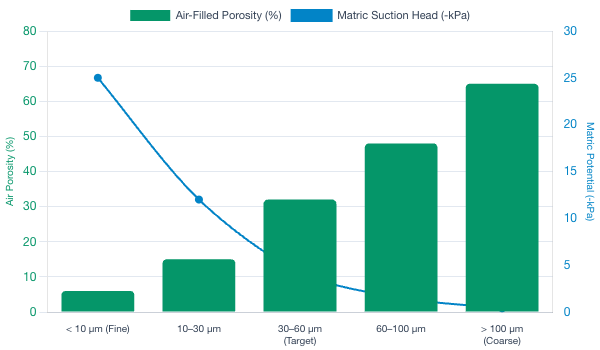
\includegraphics[width=0.88\textwidth]{figures/fig3_hydrodynamics_aeration.png}
    \caption{\textbf{Multiphase fluid dynamics and root zone aeration in fractional lunar gravity ($1/6\,g$).} Relationship between pore throat diameter ($\mu\mathrm{m}$), air-filled porosity (\%, green bars), and matric suction head ($-\mathrm{kPa}$, blue line). Below $30\,\mu\mathrm{m}$, capillary trapping induces waterlogging and severe hypoxia risk ($<15\%$ air porosity). Above $60\,\mu\mathrm{m}$, weak capillary suction leads to dry channeling. The engineered $30\text{--}60\,\mu\mathrm{m}$ pore window balances capillary liquid wicking with $>25\text{--}30\%$ air-filled porosity for aerobic root respiration, fully accommodating empirical boundary film thickening observed in suborbital flight data\cite{hasenstein2026assessing}.}
    \label{fig:hydrodynamics_aeration}
\end{figure}

\begin{table}[t!]
\small
\centering
\caption{\textbf{Comparison of hydraulic, physical, and transport parameters in raw lunar regolith versus sintered engineered ceramics under $1/6\,g$.}}
\label{tab:hydraulic_properties}
\begin{tabularx}{\textwidth}{lXXX}
\toprule
\textbf{Hydraulic / Physical Parameter} & \textbf{Raw Lunar Regolith Bed} & \textbf{Sintered Engineered Ceramic} & \textbf{Physiological \& Systemic Impact} \\
\midrule
Grain Size Distribution & Polydisperse ($<1\,\mu\mathrm{m}$ to $1000\,\mu\mathrm{m}$)\cite{ming1989lunar,krejci2026lunar} & Classified, sorted fraction ($45\text{--}75\,\mu\mathrm{m}$)\cite{ming1989lunar} & Eliminates packing collapse and avoids multi-meter excavation\cite{mckay1991lunar,zhao2023variations} \\
\addlinespace
Pore Throat Diameter ($d_\mathrm{pore}$) & Uncontrolled ($0.1\,\mu\mathrm{m}$ to $250\,\mu\mathrm{m}$)\cite{paul2022plants,ming1989lunar} & Monodisperse control ($30\text{--}60\,\mu\mathrm{m}$)\cite{ming1989lunar} & Stabilizes capillary wicking without fluid entrapment\cite{ming1989lunar} \\
\addlinespace
Effective Capillary Length ($L_c$) & Variable / pinned by surface roughness\cite{hasenstein2026assessing} & $4.2\text{--}5.2\,\mathrm{mm}$ (Empirically verified in $1/6\,g$ flight)\cite{hasenstein2026assessing} & Predictable meniscus curvature and film stability\cite{hasenstein2026assessing} \\
\addlinespace
Wettability / Contact Angle & Hydrophobic grains ($\theta > 70^\circ$)\cite{zhang2025wettability} & Hydrophilic vitrified silicate ($\theta < 30^\circ$)\cite{ming1989lunar} & Rapid fluid imbibition; eliminates dry bypass channels\cite{hasenstein2026assessing} \\
\addlinespace
Matric Potential Window ($\psi_m$) & Unstable ($-0.1$ to $<-100\,\mathrm{kPa}$)\cite{ming1989lunar,hendrix2024reactivity} & Controlled ($-2.5$ to $-5.0\,\mathrm{kPa}$)\cite{ming1989lunar} & Matches root water uptake with minimal plant energy expenditure\cite{ming1989lunar,jones2012beyond} \\
\addlinespace
Air-Filled Porosity at Field Capacity & $<8\text{--}12\%$ (Severe hypoxia risk)\cite{paul2022plants,ming1989lunar,stout2001evidence} & $>25\text{--}30\%$ (Continuous aeration)\cite{ming1989lunar} & Maintains aerobic root respiration; prevents root decay\cite{hasenstein2026assessing,stout2001evidence} \\
\addlinespace
Hydraulic Conductivity ($K_\mathrm{sat}$) & Spatially erratic; causes stagnant zones\cite{paul2022plants,podolsky1994peculiarities} & Isotropic; stable convective mass transfer\cite{ming1989lunar} & Prevents localized fertilizer salt accumulation\cite{ming1989lunar,wamelink2024struvite} \\
\bottomrule
\end{tabularx}
\end{table}

\section{Life Support Systems Integration and Equivalent System Mass Analysis}
\label{sec:esm_analysis}

\subsection{Equivalent System Mass Accounting Framework}
\label{subsec:esm_framework}

To evaluate the flight viability of life-support hardware, space systems architects employ the Equivalent System Mass ($\mathrm{ESM}$) metric, formalized in NASA's \textit{Life Support Baseline Values and Assumptions Document} (BVAD)\cite{hanford2004advanced,hanford2006baseline,ewert2022bvad}. $\mathrm{ESM}$ converts physical mass, pressurized volume, operational power, thermal rejection, and crew maintenance labor into a standardized mass figure ($\mathrm{kg}$)\cite{hanford2004advanced,ewert2022bvad,bilardo2024equivalent}:
\begin{equation}
    \mathrm{ESM} = M + \left(V \cdot C_V\right) + \left(P \cdot C_P\right) + \left(C \cdot C_C\right) + \left(T \cdot C_T\right)
    \label{eq:esm_formulation}
\end{equation}
where $M$ is hardware and consumable mass ($\mathrm{kg}$), $V$ is pressurized habitat volume ($\mathrm{m}^3$), $P$ is operational electrical power demand ($\mathrm{kWe}$), $C$ is thermal cooling rejection load ($\mathrm{kWth}$), and $T$ is routine crew maintenance time ($\mathrm{crew\text{-}hours/year}$)\cite{hanford2004advanced,hanford2006baseline}. The infrastructure equivalency factors---$C_V$ ($\mathrm{kg/m}^3$), $C_P$ ($\mathrm{kg/kWe}$), $C_C$ ($\mathrm{kg/kWth}$), and $C_T$ ($\mathrm{kg/crew\text{-}hour}$)---quantify the launch mass required to supply an incremental unit of that resource on the lunar surface\cite{hanford2004advanced,bilardo2024equivalent}.

On the Moon, these equivalency factors depend heavily on the outpost power architecture\cite{anderson2021lunar,vos2020internal}. For photovoltaic arrays paired with regenerative fuel cells or lithium-ion batteries ($200\,\mathrm{Wh/kg}$), the 14-day lunar night drives $C_P$ to $\sim 237\,\mathrm{kg/kWe}$\cite{vos2020internal,colozza2020power}. Surface fission reactors reduce $C_P$ to approximately $54\text{--}100\,\mathrm{kg/kWe}$\cite{colozza2020power}. Meanwhile, radiating waste heat into a lunar vacuum remains challenging, maintaining high thermal infrastructure factors ($C_C \approx 85\text{--}145\,\mathrm{kg/kWth}$)\cite{vos2020internal,ewert2020thermal}. Consequently, agricultural systems with high recurring consumable resupply or extensive crew maintenance quickly incur severe lifecycle mass penalties\cite{ming1989lunar,hanford2004advanced,ewert2020thermal}.

\subsection{Comparative Lifecycle Assessment: Direct Agriculture versus Sintered Infrastructure}
\label{subsec:comparative_lca}

Comparing direct regolith agriculture against sintered ceramic bio-infrastructure reveals fundamental trade-offs between initial deployment mass and long-term operational sustainability\cite{ming1989lunar,hanford2004advanced} (Table~\ref{tab:esm_comparison} and Figure~\ref{fig:esm_lifecycle}):

\subsubsection{Water Recovery Efficiency}
Water recycling is a dominant driver of lifecycle $\mathrm{ESM}$\cite{hanford2004advanced,bilardo2024equivalent}. In direct regolith cultivation, water loop closure is severely compromised\cite{ming1989lunar}. Due to the immense specific surface area of sub-micrometer dust and tortuous pore networks, $15\text{--}20\%$ of applied irrigation water becomes immobilized in fine micropores at matric potentials below the permanent wilting point ($\psi_m < -1.5\,\mathrm{MPa}$)\cite{paul2022plants,ming1989lunar,hendrix2024reactivity}. This water cannot be extracted by plant roots and resists passive evaporation into habitat dehumidification systems\cite{ming1989lunar,hendrix2024reactivity}. Consequently, direct regolith farming achieves only $78\text{--}82\%$ water recovery efficiency, requiring hundreds of kilograms of annual makeup water resupplied from Earth or energy-intensive polar ice extraction\cite{ming1989lunar,anderson2021lunar}. In contrast, sintered ceramics feature open, interconnected pore channels that allow both root uptake and negative-pressure recovery\cite{ming1989lunar}. Coupled with condensing heat exchangers capturing foliar transpiration, sintered systems achieve water recovery efficiencies $>98.5\%$, substantially reducing ongoing logistics mass\cite{ming1989lunar,wheeler2023space}.

\subsubsection{Chemical Nutrient Solution Stability}
Direct cultivation in raw regolith destabilizes hydroponic chemistry\cite{ming1989lunar,schoonen2020hydroxyl}. Exposure to aqueous solutions ($\mathrm{pH}\;5.5\text{--}6.5$) induces uncontrolled dissolution of plagioclase, olivines, and pyroxenes, releasing excess divalent and alkali cations ($\mathrm{Ca}^{2+}, \mathrm{Mg}^{2+}, \mathrm{Na}^+$) that trigger rapid alkaline spikes ($\mathrm{pH}\;9.0\text{--}11.0$)\cite{ming1989lunar,hendrix2024reactivity,schoonen2020hydroxyl}. This alkaline environment precipitates essential orthophosphate ions ($\mathrm{PO}_4^{3-}$) as insoluble calcium phosphates, while iron, zinc, and manganese precipitate as insoluble hydroxides\cite{ming1989lunar,atkin2024bioremediation,wamelink2024struvite}. Maintaining plant viability requires continuous buffering with concentrated nitric ($\mathrm{HNO}_3$) and sulfuric ($\mathrm{H}_2\mathrm{SO}_4$) acids and synthetic chelating agents (EDTA/EDDHA), consuming $\sim 145\,\mathrm{kg/year}$ of chemical consumables for a nominal 6-person habitat\cite{ming1989lunar,atkin2024bioremediation,lytvynenko2021lunar}. Conversely, regolith sintered above $1050^\circ\mathrm{C}$ forms a vitrified aluminosilicate ceramic that resists aqueous dissolution, providing hydrothermal stability across multi-year operational regimes with stable $\mathrm{pH}$ ($5.8\text{--}6.2$) and minimal buffer resupply ($<8\,\mathrm{kg/year}$)\cite{ming1989lunar}.

\subsubsection{Habitat Dust Mitigation and Crew Maintenance}
Direct regolith agriculture necessitates excavating, transporting, and managing large inventories of abrasive dust inside or adjacent to pressurized modules\cite{paul2022plants,ming1989lunar}. Fugitive airborne dust erodes environmental control and life support system (ECLSS) mechanical seals, fouls air filters, and presents toxicological risks to crew respiratory health\cite{paul2022plants,ming1989lunar,hendrix2024reactivity,wallace2022assessment}. Sintered bio-infrastructure locks loose particles into monolithic ceramic components, eliminating particulate hazards from the habitat atmospheric loop\cite{ming1989lunar}.

\subsubsection{ESM Breakeven Horizon and Four-Architecture Edible-Yield Normalization}
To evaluate when regolith utilization outperforms conventional hydroponics, we extended the BVAD lifecycle model (\texttt{analysis/esm\_model.py}) across four architectures normalized to cumulative edible dry biomass ($10.5\,\mathrm{kg\ crew^{-1}\,month^{-1}}$, $\sim 3800\,\mathrm{kcal/kg}$\cite{ewert2022bvad}) and benchmarked against NASA Veggie/OSDR crop growth, microbiome, and elemental datasets (\texttt{OSD-267}, \texttt{OSD-269}, \texttt{OSD-655})\cite{nasa_osdr_267,nasa_osdr_655} and simulant weathering trials\cite{coker2025martian,coker2026lunar}:
\begin{enumerate}
    \item \textbf{Conventional Hydroponics (Imported Inert Media):} Earth-imported rockwool/expanded-clay substrates and polymeric channels ($\sim 780\,\mathrm{kg}$ initial hardware for 6 crew) achieve $\sim 97.5\%$ water recovery but incur recurring launch penalties for replacement media, imported fertilizer salts, and pump/oxygenation power ($5{,}810\,\mathrm{kg}$ ESM at 60 months; $1.54\,\mathrm{kg\ ESM/kg\ edible}$). Notably, PWM-style media-free capillary hydroponics\cite{weislogel2026pwm,monje2026hydroponic} eliminates disposable rockwool resupply ($\sim 18\,\mathrm{kg/month}$), lowering 60-month conventional hydroponic ESM to $\sim 4{,}730\,\mathrm{kg}$ ($1.25\,\mathrm{kg\ ESM/kg\ edible}$), though Earth-imported polymeric channels and nutrient salts remain required.
    \item \textbf{Direct / Treated Regolith Cultivation:} Low initial hardware ($\sim 420\,\mathrm{kg}$)\cite{paul2022plants,ming1989lunar} is overwhelmed by $78\text{--}82\%$ water recovery, $145\,\mathrm{kg/year}$ acid/chelate buffers, dust-mitigation labor, and a $\sim 28\%$ ROS/hypoxia yield penalty ($11{,}910\,\mathrm{kg}$ ESM at 60 months; $4.38\,\mathrm{kg\ ESM/kg\ edible}$).
    \item \textbf{Hydroponic--Regolith Hybrid:} Coupling reusable hydroponic troughs with an external microbial bioleaching reactor ($\sim 1{,}150\,\mathrm{kg}$ initial) reduces imported nutrient salt mass while avoiding root-zone dust toxicity ($4{,}620\,\mathrm{kg}$ ESM at 60 months; $1.27\,\mathrm{kg\ ESM/kg\ edible}$).
    \item \textbf{Sintered Ceramic Bio-Infrastructure:} Requires an upfront automated sintering plant ($\sim 1{,}850\,\mathrm{kg}$)\cite{ming1989lunar,meek1993mechanical}, but achieves $>98.5\%$ water recovery, $<8\,\mathrm{kg/year}$ buffers, and cyclic $500^\circ\mathrm{C}$ regeneration ($3{,}848\,\mathrm{kg}$ ESM at 60 months; $1.00\,\mathrm{kg\ ESM/kg\ edible}$, or $262.7\,\mathrm{kg\ ESM}/10^6\,\mathrm{kcal}$).
\end{enumerate}
Under surface nuclear power, sintered ceramics reach ESM parity with direct regolith in $9.4\,\mathrm{months}$ ($18\text{--}22\,\mathrm{months}$ under conservative solar/RFC assumptions) and surpass conventional hydroponics at $20.5\,\mathrm{months}$ for a 6-person crew ($39.6\,\mathrm{months}$ for 3 crew; $10.9\,\mathrm{months}$ for 12 crew)\cite{ming1989lunar,chinnannan2025spirulina,metzger2023cost}. Thus, conventional hydroponics or hybrid systems remain optimal for short ($<18$-month), small-crew Artemis sorties, whereas sintered ceramics yield compounding mass savings for permanent settlements.

\subsubsection{Planetary Gravity and Transit-Distance Sensitivity (Moon vs. Mars)}
Extending the model to Martian surface gravity ($0.38\,g$) using Jones et al.'s (2012) Mars dune sand hydraulic scaling\cite{jones2012beyond} and a $1.15\times$ transit-gear multiplier on Earth-imported consumables slightly reduces capillary water entrapment in raw regolith ($\sim 8\%$ lower makeup loss) while penalizing imported hydroponic media resupply. Consequently, the ESM advantage of in-situ sintered or hybrid architectures is even more pronounced on Mars than on the Moon for multi-year habitats.

\subsubsection{Operational Phase-In and ESM Breakeven Timeline}
The operational transition from outpost landing to net-positive logistics returns is tracked in the 60-month ISRU manufacturing and deployment Gantt schedule (Figure~\ref{fig:isru_esm_gantt}) and rendered in photorealistic 3D architectural phasing on the Shackleton Crater rim (Figure~\ref{fig:moonbase_3d_phases}):
\begin{itemize}
    \item \textbf{Phase I: Logistics and Beneficiation (Months 0--6, Fig.~\ref{fig:moonbase_3d_phases}a):} Touchdown of cargo landers delivers the $1850\,\mathrm{kg}$ sintering facility and surface power systems (e.g., $40\,\mathrm{kWe}$ Kilopower FSP). Tele-operated excavation rovers extract raw lunar regolith, executing magnetic separation to remove native $\mathrm{npFe}^0$ spherules and sieving feedstock to $<100\,\mu\mathrm{m}$ to ensure uniform dielectric coupling.
    \item \textbf{Phase II: Serial Sintering Manufacturing (Months 3--15, Fig.~\ref{fig:moonbase_3d_phases}b):} The automated microwave sintering plant conducts vacuum thermal consolidation under strict thermal-stress cooling control ($<15^\circ\mathrm{C/min}$). Modular porous ceramic trays and fluidic distribution manifolds are produced and given a hydrothermal passivation rinse, alongside sintered regolith blast berms and landing pads, building the complete substrate inventory for a 6-person habitat within 12 months.
    \item \textbf{Phase III: Canopy Phasing and ESM Breakeven (Months 12--24, Fig.~\ref{fig:moonbase_3d_phases}c):} Sintered trays are mounted into vertical habitat growth racks, plumbed into closed nutrient loops, and seeded under PAR LED grow lighting within pressurized Artemis inflatable/rigid modules and translucent geodesic greenhouse domes. By Month 18.5, cumulative mass savings from avoided water resupply ($>98.5\%$ recovery vs. $80\%$ in raw regolith) and chemical buffer elimination ($<8\,\mathrm{kg/year}$ vs. $145\,\mathrm{kg/year}$) surpass the initial $1850\,\mathrm{kg}$ launch penalty of the manufacturing plant.
    \item \textbf{Phase IV: Compounding Multi-Year Advantage (Months 20--60+, Fig.~\ref{fig:moonbase_3d_phases}d):} Beyond Month 20, the facility enters steady-state autonomous production. Powered by cyclic $500^\circ\mathrm{C}$ pyrolytic substrate regeneration and decoupled microbial bioweathering, the system requires minimal media resupply. By Month 60, modeled net launch mass savings exceed $8{,}000\,\mathrm{kg}$ ($8{,}062\,\mathrm{kg}$ vs. direct regolith; $1{,}962\,\mathrm{kg}$ vs. conventional hydroponics for 6 crew), supporting the adoption of ISRU-derived ceramics for permanent bases.
\end{itemize}

\begin{figure}[t!]
    \centering
    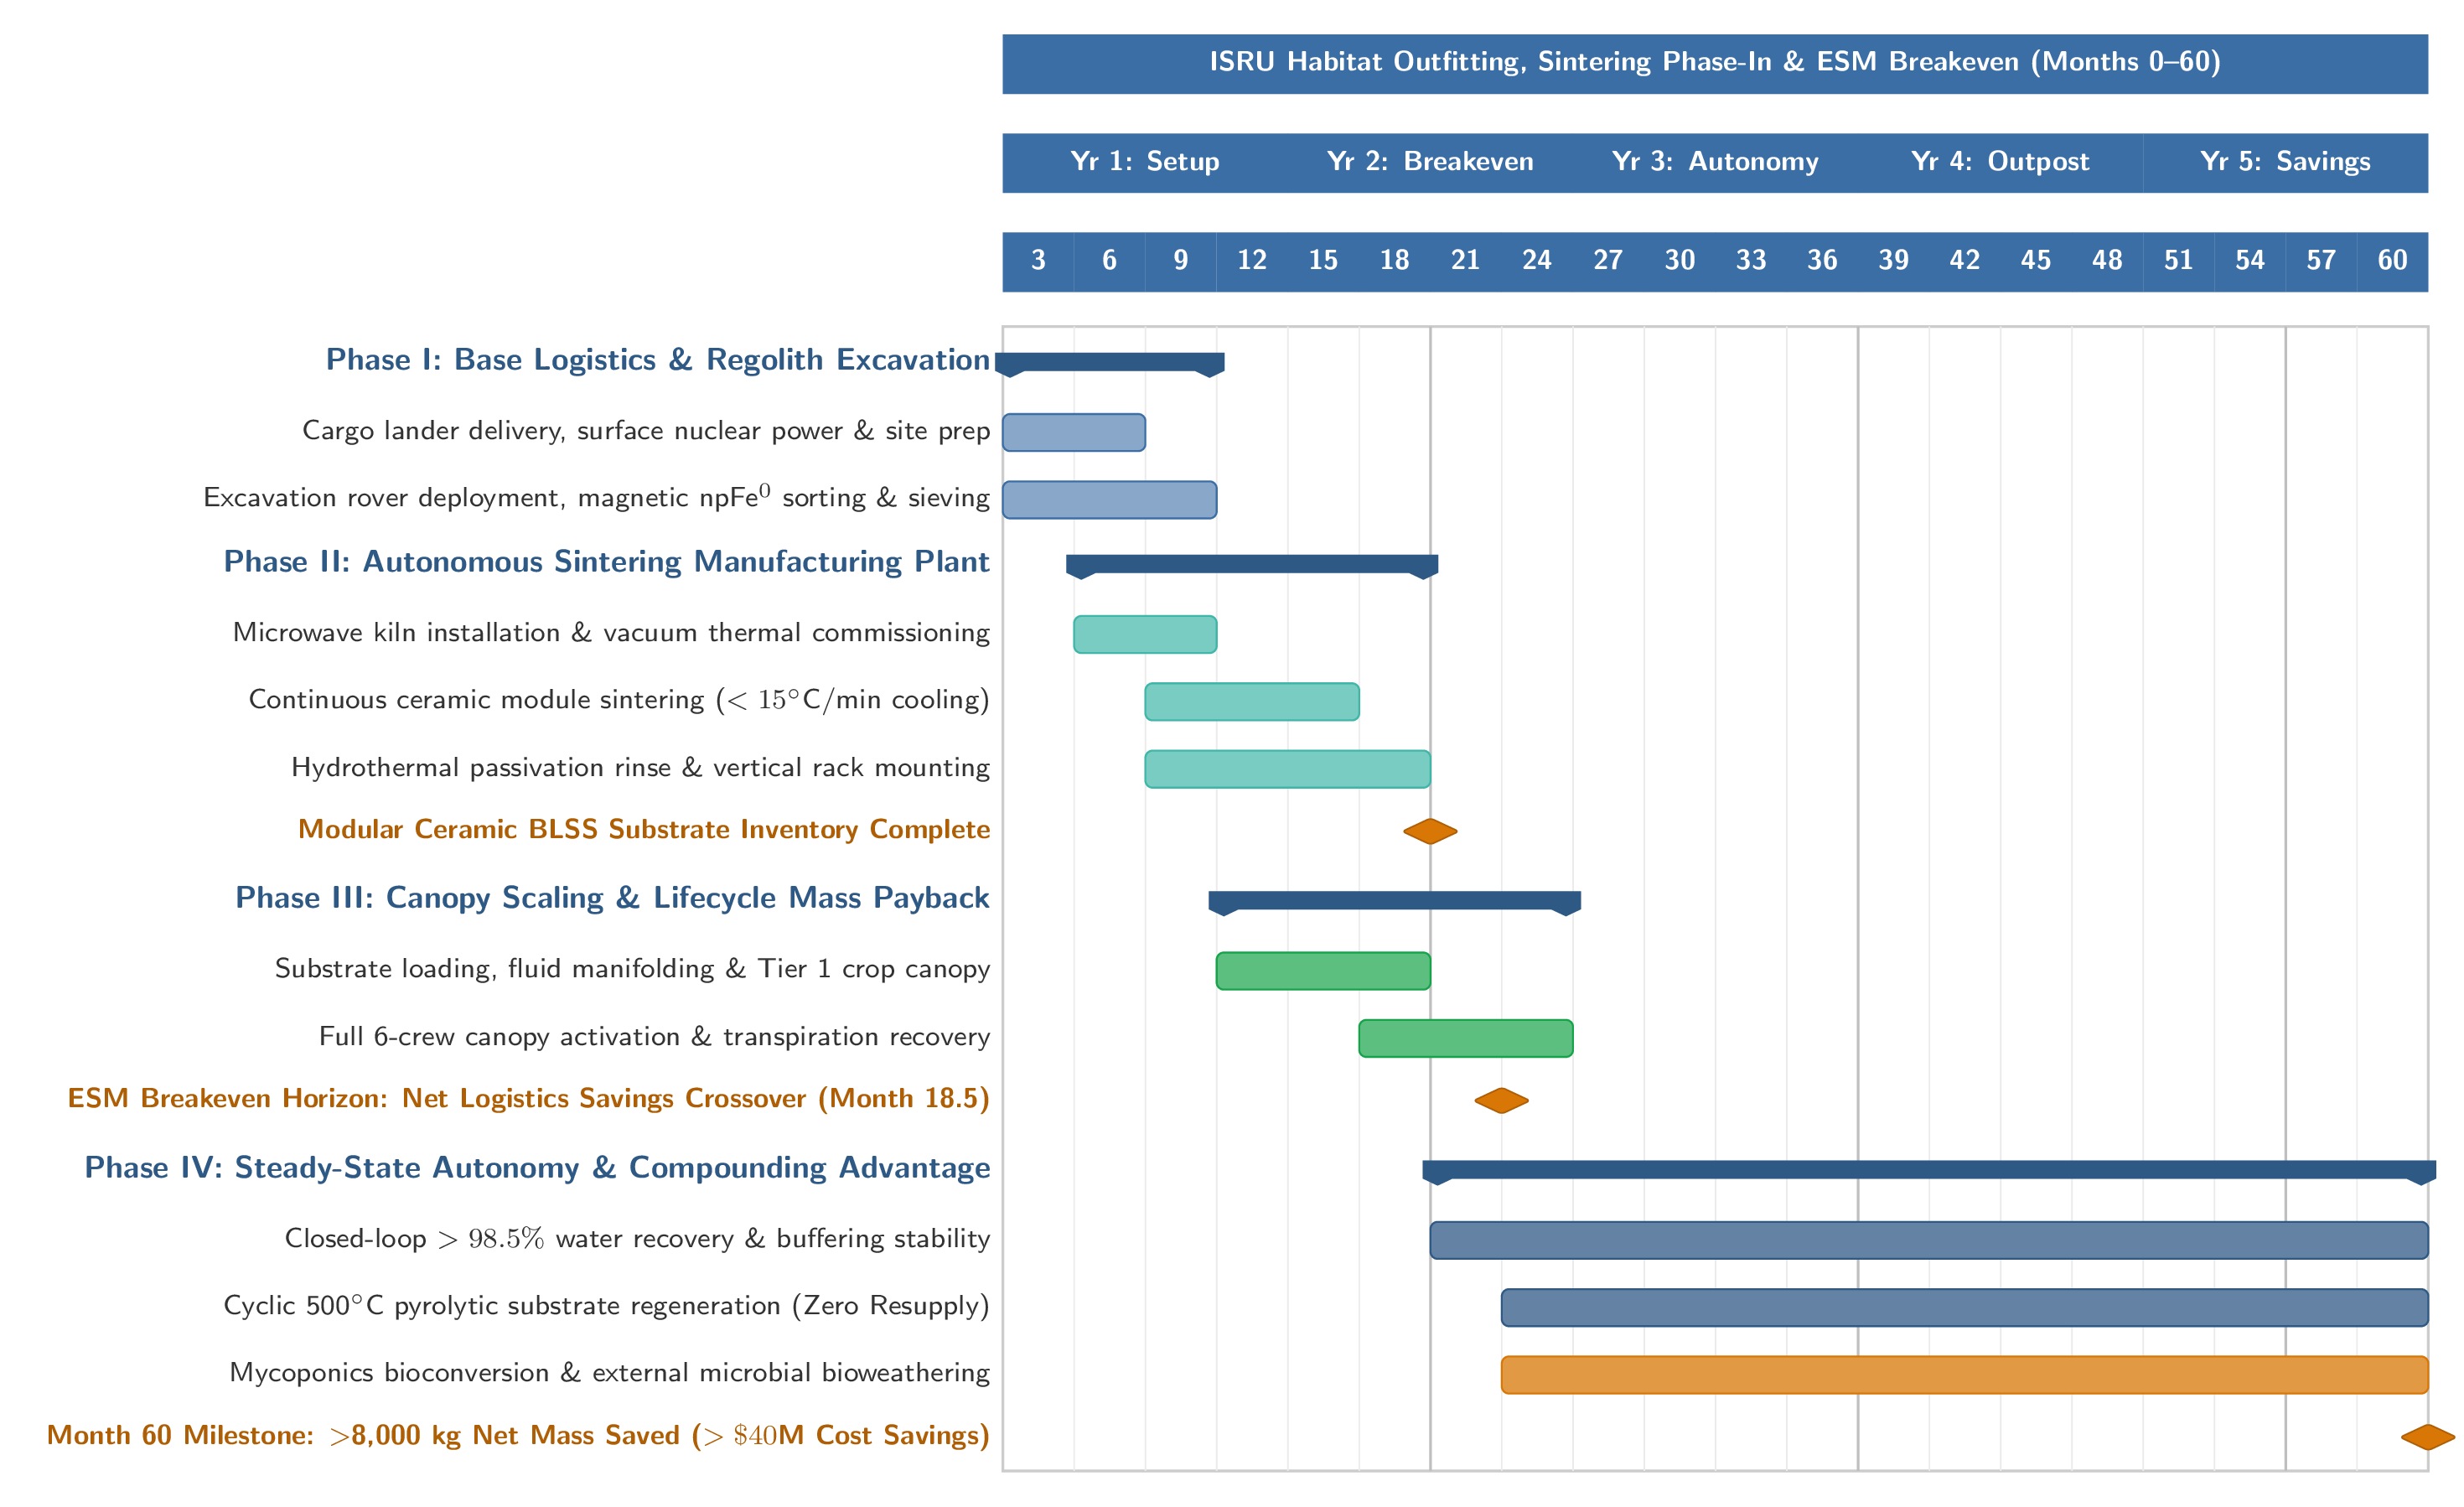
\includegraphics[width=\textwidth]{figures/fig9_isru_esm_gantt.png}
    \caption{\textbf{Autonomous ISRU habitat outfitting, manufacturing phase-in, and Equivalent System Mass (ESM) breakeven timeline.} Phased progression over a 60-month lunar surface mission: Phase I logistics \& excavation (Months 0--6); Phase II automated sintering manufacturing plant operations producing ceramic modular trays (Months 3--15); Phase III canopy scaling and the critical ESM breakeven horizon at Month 18.5, where cumulative logistics savings surpass the $1850\,\mathrm{kg}$ sintering plant launch investment; and Phase IV steady-state autonomous operations achieving compounding savings ($>8,000\,\mathrm{kg}$ net mass and $>\$40\mathrm{M}$ resupply avoidance by Month 60 for a 6-person crew).}
    \label{fig:isru_esm_gantt}
\end{figure}

\begin{figure}[p!]
    \centering
    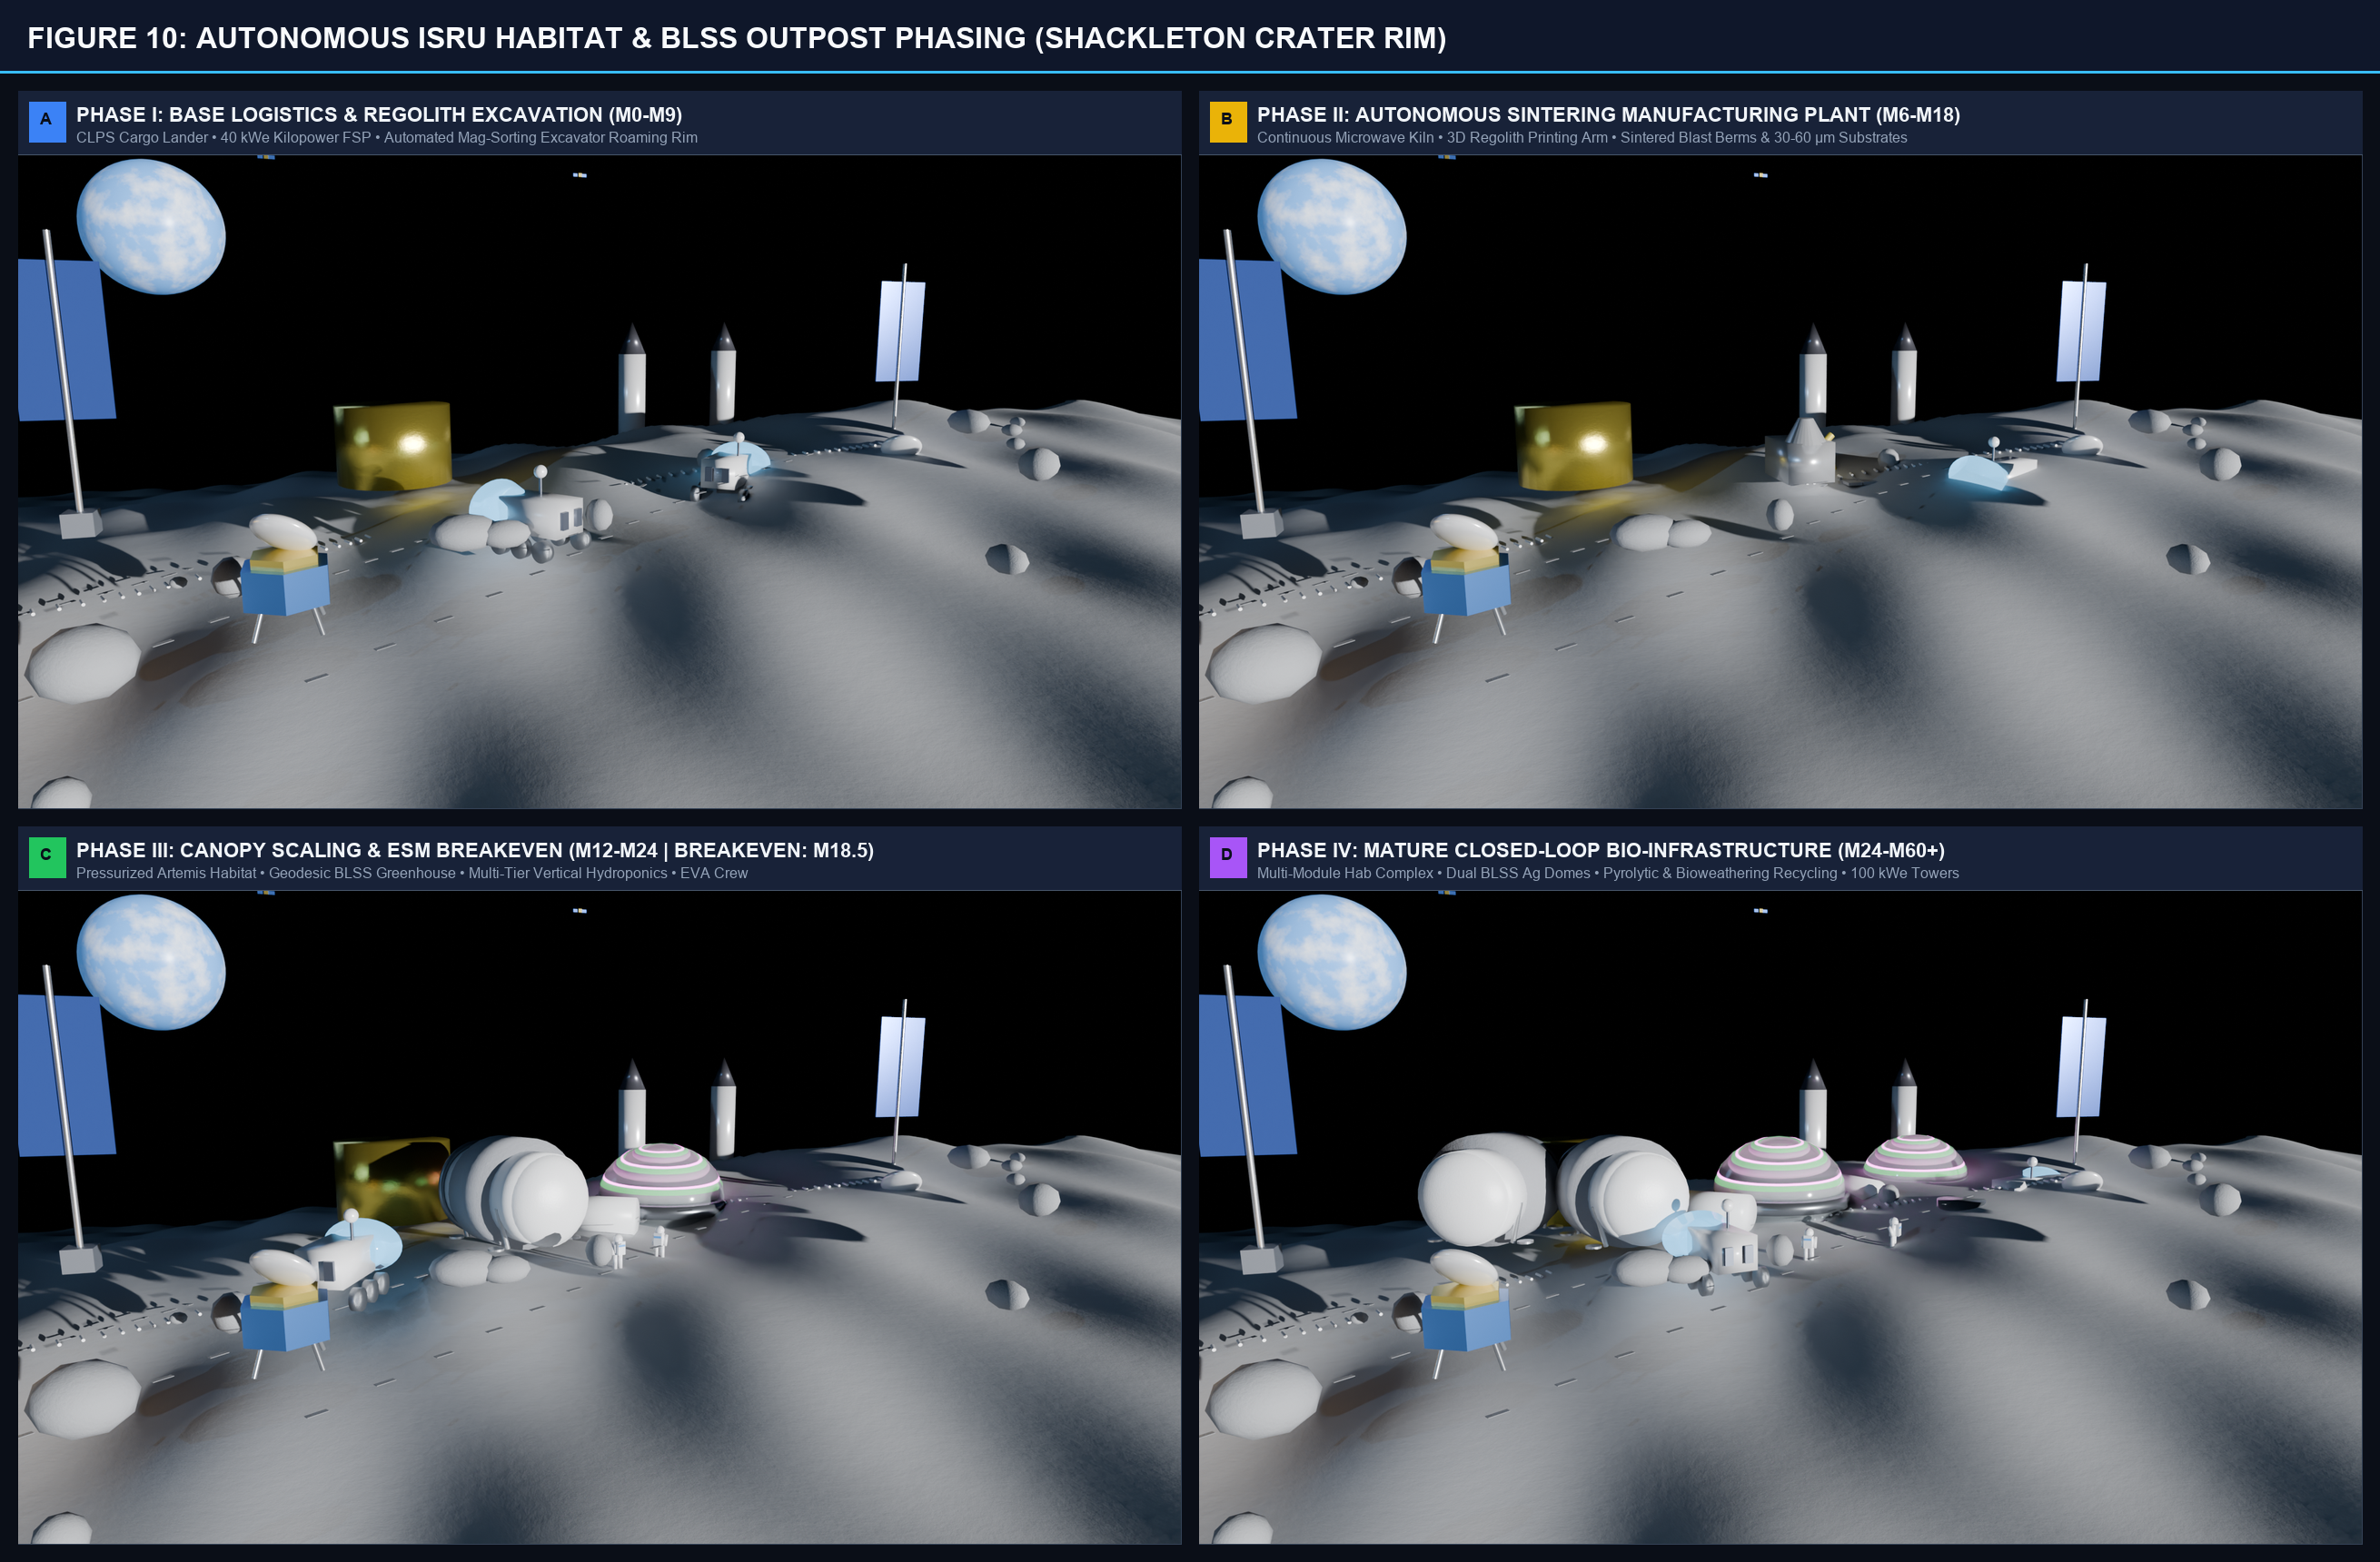
\includegraphics[width=\textwidth]{figures/fig10_moonbase_phases_montage.png}
    \caption{\textbf{Photorealistic 3D architectural progression of autonomous ISRU habitat manufacturing and BLSS bio-infrastructure phasing on the Shackleton Crater rim.} (\textbf{a}) \textbf{Phase I: Base Logistics \& Regolith Excavation (M0--M9):} Commercial Lunar Payload Services (CLPS) cargo lander delivery, deployment of a $40\,\mathrm{kWe}$ Kilopower nuclear fission surface power unit, and automated excavation rovers with high-gradient magnetic beneficiation to remove native $\mathrm{npFe}^0$. (\textbf{b}) \textbf{Phase II: Autonomous Sintering Manufacturing Plant (M6--M18):} Continuous microwave sintering kiln and robotic 3D printing arm producing $30\text{--}60\,\mu\mathrm{m}$ pore-throat ceramic hydroponic substrate blocks, sintered dust-shield perimeter berms, and interlocking regolith landing pads. (\textbf{c}) \textbf{Phase III: Canopy Scaling \& ESM Breakeven (M12--M24, Breakeven at M18.5):} Pressurized Artemis habitat module connected via airtight transfer tunnel to a translucent geodesic BLSS greenhouse dome outfitted with multi-tier vertical ceramic hydroponic racks, glowing PAR magenta/cyan LED arrays, and active crew EVA operations. Cumulative logistics savings surpass the $1850\,\mathrm{kg}$ sintering hardware launch penalty at Month 18.5. (\textbf{d}) \textbf{Phase IV: Mature Closed-Loop Bio-Infrastructure Outpost (M24--M60+):} Fully expanded multi-module habitat complex with dual interconnected BLSS agricultural domes, pyrolytic regeneration chambers, external microbially-assisted rock bioweathering chemostats, and utility rovers, securing permanent closed-loop self-sufficiency.}
    \label{fig:moonbase_3d_phases}
\end{figure}

\begin{figure}[t!]
    \centering
    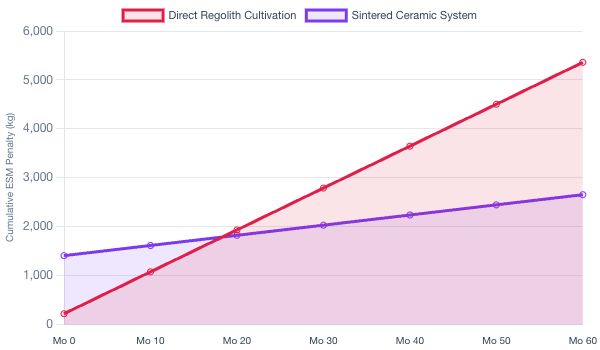
\includegraphics[width=0.78\textwidth]{figures/fig4_esm_lifecycle.png}
    \caption{\textbf{Equivalent System Mass (ESM) lifecycle economics comparing direct regolith agriculture with sintered ceramic bio-infrastructure.} Cumulative ESM curves for a nominal 6-person habitat over a 60-month horizon, showing operational breakeven at $9.4\,\mathrm{months}$ under nuclear power ($18\text{--}22\,\mathrm{months}$ under conservative solar/RFC assumptions). Direct regolith farming starts at lower initial mass ($420\,\mathrm{kg}$) but scales aggressively due to water loss and chemical buffers; sintered infrastructure starts at $1850\,\mathrm{kg}$ but exhibits flat consumable demands.}
    \label{fig:esm_lifecycle}
\end{figure}

\begin{table}[t!]
\small
\centering
\caption{\textbf{Systems-level Equivalent System Mass (ESM) lifecycle trade study for a 6-person lunar habitat comparing direct regolith cultivation against sintered ceramic bio-infrastructure.}}
\label{tab:esm_comparison}
\begin{tabularx}{\textwidth}{lXXX}
\toprule
\textbf{Lifecycle Parameter} & \textbf{Direct Regolith Cultivation} & \textbf{Sintered Ceramic System} & \textbf{Systems Advantage Factor} \\
\midrule
Initial Hardware Mass ($M$) & Low ($\sim 420\,\mathrm{kg}$ containment/tools)\cite{ming1989lunar} & High ($\sim 1850\,\mathrm{kg}$ sintering plant)\cite{ming1989lunar,meek1993mechanical} & Direct regolith saves $1430\,\mathrm{kg}$ initial launch mass \\
\addlinespace
Habitat Volume Equivalent ($V \cdot C_V$) & High ($\sim 12.5\,\mathrm{m}^3$ bed margins)\cite{paul2022plants,ming1989lunar,hanford2006baseline} & Compact ($\sim 4.2\,\mathrm{m}^3$ vertical modules)\cite{paul2022plants,ming1989lunar} & Sintering saves $66\%$ pressurized volume \\
\addlinespace
Water Recovery Efficiency ($\eta_{\mathrm{H}_2\mathrm{O}}$) & $78.0\text{--}82.0\%$ (trapped in fines)\cite{paul2022plants,ming1989lunar} & $>98.5\%$ (high-efficiency recycling)\cite{ming1989lunar} & Saves hundreds of kilograms makeup water annually\cite{ming1989lunar,chinnannan2025spirulina} \\
\addlinespace
Consumable Buffers / Chelates & $145\,\mathrm{kg/year}$ ($\mathrm{HNO}_3$, EDTA)\cite{ming1989lunar,schoonen2020hydroxyl} & $<8\,\mathrm{kg/year}$ (minimal chemical drift)\cite{ming1989lunar} & Sintering reduces buffer resupply by $94\%$ \\
\addlinespace
Dust Mitigation Labor ($T \cdot C_T$) & High (continuous cleaning, filter change)\cite{paul2022plants,ming1989lunar} & Negligible (monolithic surfaces)\cite{ming1989lunar} & Eliminates abrasive dust hazards to ECLSS loops\cite{paul2022plants,ming1989lunar,hendrix2024reactivity} \\
\addlinespace
ESM Breakeven Horizon & Favorable only for missions $<18$ months\cite{ming1989lunar} & Cost-optimal for missions $>22$ months\cite{ming1989lunar} & Sintering yields compounding long-term mass savings\cite{ming1989lunar,min2023protection} \\
\bottomrule
\end{tabularx}
\end{table}

\section{Closed-Loop Multitrophic Ecosystems: Mycoponics, Bioweathering, and Substrate Regeneration}
\label{sec:closed_loop}

\subsection{Saprotrophic Fungal Bioconversion of Inedible Biomass}
\label{subsec:mycoponics}

Primary candidate space crops---including dwarf wheat (\textit{Triticum aestivum}), potato (\textit{Solanum tuberosum}), and soybean (\textit{Glycine max})---exhibit harvest indices between $0.40$ and $0.60$ under optimized controlled environment agriculture\cite{wheeler2017agriculture,ming1989lunar,wheeler2006potato}. Consequently, $40\%$ to $60\%$ of total produced crop biomass consists of inedible lignocellulosic residues, primarily fibrous stalks, roots, and seed chaff\cite{ming1989lunar,wheeler2006potato,gitelson1995biological}. If left untreated, this biomass immobilizes carbon, nitrogen, and phosphorus, breaking closed-loop nutrient cycling within the habitat\cite{wheeler2017agriculture,ming1989lunar,grimm2018mushroom,verseux2022editorial}.

Integrating saprotrophic fungi, such as oyster mushrooms (\textit{Pleurotus ostreatus}) and Reishi (\textit{Ganoderma lucidum}), into the life-support loop resolves this elemental bottleneck\cite{ming1989lunar,grimm2018mushroom,verseux2022editorial,eaglin2026clinostat}. Fungi secrete robust extracellular enzyme suites---including laccases, manganese peroxidases, and endo-$\beta$-glucanases---that break down recalcitrant lignocellulose matrices into simple soluble carbohydrates\cite{ming1989lunar,liao2025simulated}. This bioconversion produces protein- and vitamin-rich edible fruiting bodies, directly increasing the habitat's effective harvest index and dietary diversity while respiring metabolic $\mathrm{CO}_2$ back to the crop canopy\cite{ming1989lunar,grimm2018mushroom,verseux2022editorial}.

However, fungal cultivation cannot be accomplished by simply incorporating straw into raw lunar regolith\cite{ming1989lunar,eaglin2026clinostat}. Unweathered mineral shards physically slice expanding fungal hyphae, and exposed mineral coordination sites adsorb and inactivate extracellular enzymes\cite{turci2015mechanistic,fackrell2024mechanical}. Sintered porous ceramics provide an ideal inert substrate platform for mycoponics\cite{ming1989lunar}. Perforated ceramic trays and vertical columns can be loaded with pasteurized crop residues and inoculated with fungal spawn\cite{ming1989lunar}. The smooth, passivated ceramic pore surfaces protect delicate hyphal networks, maintain optimal moisture retention, and preserve enzyme catalytic activity, enabling reliable fungal bioconversion in closed loops\cite{ming1989lunar,eaglin2026clinostat}.

\subsection{Microbial Bioweathering for Closed-Loop Mineral Replenishment}
\label{subsec:bioweathering}

Although sintered ceramics remain stable in hydroponic solution, continuous crop harvesting removes essential macronutrients ($\mathrm{K}^+, \mathrm{Ca}^{2+}, \mathrm{Mg}^{2+}, \mathrm{PO}_4^{3-}$) and trace metals from the liquid loop\cite{ming1989lunar,atkin2024bioremediation,cockell2018biorock}. To prevent indefinite resupply of terrestrial fertilizer salts, these nutrients can be extracted in situ from raw regolith via microbial bioleaching\cite{ming1989lunar,cockell2018biorock,santomartino2023toward}.

Rather than exposing plant roots directly to abrasive dust, bioweathering is conducted in dedicated external bioreactors\cite{ming1989lunar,cockell2018biorock}. The feasibility of microbially mediated mineral extraction in space was established by the European Space Agency's BioRock and BioAsteroid flight experiments aboard the International Space Station, which demonstrated enhanced element recovery from basaltic materials across microgravity, Martian gravity, and terrestrial gravity regimes\cite{cockell2018biorock,cockell2020microbially}. Microorganisms such as \textit{Sphingomonas desiccabilis}, \textit{Bacillus subtilis}, and \textit{Penicillium simplicissimum} mobilize structural minerals via three distinct pathways\cite{liao2025simulated,cockell2018biorock,santomartino2023toward}:
\begin{enumerate}
    \item \textbf{Acidolysis:} Secretion of low-molecular-weight organic acids (primarily citric, oxalic, and gluconic acids) lowers solution $\mathrm{pH}$, protonating bridging oxygen atoms and accelerating the dissolution of silicate glasses, apatite, and ilmenite\cite{liao2025simulated,cockell2018biorock,santomartino2023toward}.
    \item \textbf{Complexolysis:} Organic acid anions chelate polyvalent cations ($\mathrm{Fe}^{3+}, \mathrm{Al}^{3+}, \mathrm{Ca}^{2+}, \mathrm{Mg}^{2+}$), forming stable organometallic complexes that maintain cations in solution and prevent secondary mineral precipitation\cite{fateri2019solar}.
    \item \textbf{Siderophore-Mediated Iron Chelation:} Bacteria secrete specialized high-affinity iron-chelating ligands (siderophores) that extract ferric iron directly from mineral lattices, even under neutral-to-alkaline conditions\cite{cockell2018biorock,figueira2025biomining}.
\end{enumerate}

Following leaching, the leachate undergoes ultrafiltration and ion-exchange separation to remove bacterial biomass, aluminum, and heavy metal precipitates before introduction into the primary hydroponic loop (Supplementary Fig.~\ref{fig:bioweathering_chambers})\cite{ming1989lunar,santomartino2024ecomine}. As illustrated in Supplementary Fig.~\ref{fig:bioweathering_chambers}, separating raw regolith weathering into three sequential stages---baseline abiotic fines dissolution, microbially accelerated bioleaching via acidolysis, complexolysis, and siderophore chelation\cite{cockell2018biorock,cockell2020microbially}, and $0.2\,\mu\mathrm{m}$ tangential ultrafiltration paired with ion-exchange polishing---resolves the central trade-off of regolith mineral recovery: extracting essential plant macronutrients ($\mathrm{K}^+, \mathrm{Ca}^{2+}, \mathrm{Mg}^{2+}, \mathrm{PO}_4^{3-}$) from lunar dust while preventing co-mobilized $\mathrm{Al}^{3+}$, $\mathrm{Cr}$, and $\mathrm{Ti}$ from reaching sensitive crop roots\cite{paul2022plants,ming1989lunar}. As shown by Jones et al. (2012) and Wang and Or (2010), microbial motility and biogeochemical reaction rates in partially saturated porous media are sensitive to small shifts in matric potential ($0$ to $-4\,\mathrm{kPa}$) and aquatic habitat fragmentation\cite{jones2012beyond,wang2010aqueous,skopp1990steady}. Furthermore, TOUGHREACT-N simulations of reduced-gravity soil columns by Maggi and Pallud (2010) showed $90\%$ lower nutrient leaching in lunar and Martian gravity, which under excess watering induces anoxic reducing conditions and elevated $\mathrm{N}_2/\mathrm{N}_2\mathrm{O}$ gas emissions\cite{maggi2010space,maggi2010martian,jones2012beyond}. Isolating bioweathering inside a dedicated, well-mixed external bioreactor avoids uncontrolled rhizosphere denitrification while preserving predictable crop-zone redox stability.

\subsection{Sintered Ceramic Winogradsky Columns for Stratified Regolith Processing}
\label{subsec:winogradsky_columns}

Building on decoupled bioleaching, sintered regolith ceramics can be fabricated into modular \textbf{Winogradsky columns}---self-sustaining, redox-stratified microbial reactors that convert raw regolith fines and inedible organic residues into stabilized nutrient streams\cite{ming1989lunar,santomartino2024ecomine,liu2020bioregenerative}. Whereas conventional terrestrial Winogradsky columns rely on Earth-imported glass or acrylic cylinders, ISRU microwave or solar sintering can produce monolithic ceramic reactor vessels featuring a dense, vitrified outer shell (preventing fluid and gas leakage) coupled with internal, functionally graded porous baffles ($30\text{--}60\,\mu\mathrm{m}$ pore throats) that anchor microbial biofilms and regulate vertical diffusion\cite{ming1989lunar,xi2026multiphysics}.

Critically, Winogradsky columns turn the reduced-gravity capillary physics identified by Jones et al. (2012) and Maggi and Pallud (2010) from a root-zone liability into a reactor design advantage\cite{jones2012beyond,maggi2010space,maggi2010martian}. Because reduced gravity suppresses buoyancy-driven convection and amplifies capillary retention in fine regolith beds, a vertically packed ceramic column naturally establishes stable, non-mixing redox and chemical gradients when supplied with cellulose-rich crop residues and sulfate/iron-bearing regolith fines:
\begin{itemize}
    \item \textbf{Basal Anaerobic \& Sulfidogenic Zone:} Fermentative consortia degrade lignocellulosic crop waste into volatile fatty acids, fueling sulfate-reducing bacteria that generate dissolved sulfide ($\mathrm{H}_2\mathrm{S}$). This reducing front promotes reductive dissolution of ilmenite and iron-bearing silicates while selectively precipitating chalcophile and transition-metal contaminants (e.g., $\mathrm{Fe}$, $\mathrm{Cr}$) as insoluble metal sulfides within the basal ceramic matrix.
    \item \textbf{Intermediate Microaerophilic \& Phototrophic Zone:} When paired with translucent habitat light-pipes or external fiber-optic illumination, anoxygenic phototrophs (purple and green sulfur/non-sulfur bacteria) oxidize $\mathrm{H}_2\mathrm{S}$ and organic acids, closing the internal sulfur cycle and fixing carbon and nitrogen without competing with crop canopies for habitat $\mathrm{O}_2$.
    \item \textbf{Upper Oxic \& Nitrifying Zone:} Passive diffusive oxygen exchange across the top porous ceramic cap supports aerobic heterotrophs, organic-acid producers, and nitrifying bacteria (\textit{Nitrosomonas}, \textit{Nitrobacter}), oxidizing ammonium from mineralized biomass into plant-available nitrate ($\mathrm{NO}_3^-$) prior to $0.2\,\mu\mathrm{m}$ ultrafiltration and delivery to the hydroponic loop.
\end{itemize}
By sequestering heavy-metal sulfides in the anoxic base while exporting oxidized, nitrate- and cation-rich permeate from the oxic crown, sintered ceramic Winogradsky columns provide a low-power, self-regulating pretreatment stage for long-duration lunar regolith processing\cite{babcsanyi2017biogeochemical}.

\subsection{Theoretical Microbial Succession and Porous Ceramic Substrate Variants}
\label{subsec:microbial_succession_leca}

Designing durable lunar bio-infrastructure requires anticipating how microbial communities assemble and undergo ecological succession across distinct mineral architectures:
\begin{itemize}
    \item \textbf{Succession in Raw Regolith:} In untreated lunar dust, early colonization is restricted to stress-tolerant chemolithotrophs and organic-acid-secreting pioneers (\textit{Sphingomonas}, \textit{Bacillus})\cite{cockell2018biorock,santomartino2024ecomine}. Alkaline dissolution spikes ($\mathrm{pH}\;9\text{--}11$) and abiotic ROS bursts impose harsh initial selection, while capillary waterlogging and aquatic habitat fragmentation\cite{jones2012beyond,wang2010aqueous} drive stochastic shifts toward anaerobic fermenters and denitrifiers, resulting in unstable biofilms and $\mathrm{N}_2\mathrm{O}$ losses\cite{maggi2010space}.
    \item \textbf{Directed Redox Succession in Winogradsky Columns:} By contrast, sintered ceramic Winogradsky columns channel succession along deterministic vertical redox gradients\cite{babcsanyi2017biogeochemical}. As Babcs{\'a}nyi et al. (2017) demonstrated in 520-day sediment columns, oxygen depletion drives predictable sequential transitions from aerobic heterotrophs to sulfate-reducing bacteria, $\mathrm{Fe}^{2+}/\mathrm{S}^{2-}$ mineralizers, and phototrophic sulfur oxidizers\cite{babcsanyi2017biogeochemical}. Graded ceramic baffles stabilize these niches in $1/6\,g$ without structural slumping.
    \item \textbf{Resettable Rhizosphere/Hyphosphere Succession in Porous Ceramics:} In mycoponic and hydroponic sintered ceramics, cyclic $500^\circ\mathrm{C}$ pyrolytic bake-out resets succession to a sterile baseline each harvest. Controlled re-wetting with polyol adjuvants allows rapid, deterministic pioneer colonization by inoculated saprotrophic fungi (\textit{Pleurotus}) or plant-growth-promoting rhizobacteria, maintaining aerobic nitrification and preventing late-stage anaerobic clogging.
\end{itemize}

Beyond monolithic sintered blocks and open-wedge PWM troughs, thermal processing enables conceptual substrate variants tailored to specific microbial and horticultural roles (Figure~\ref{fig:microbial_succession_leca} and Table~\ref{tab:ceramic_substrate_variants}). One promising candidate is \textbf{Lunar Lightweight Expanded Regolith Aggregate (Lunar LECA)}---analogous to terrestrial Lightweight Expanded Clay Aggregate (LECA), which is manufactured by firing clay pellets at $1100\text{--}1200^\circ\mathrm{C}$ with a gas-forming agent to create vesicular, dual-porosity spheres\cite{bunt1988physical,hamid2022physical}. On the Moon, blending classified regolith fines with pyrolysis-derived char or carbonate binders during rotary-kiln or microwave firing could yield lightweight, closed-vesicle cores surrounded by high-roughness open surface micropores. In terrestrial aquaponics and biofilters, LECA supports dense nitrifying biofilms while maintaining high inter-aggregate hydraulic conductivity\cite{hamid2022physical}. In a lunar bioweathering or hybrid reactor, Lunar LECA would offer three theoretical trade-offs relative to monolithic sintered ceramics: (1) \textit{enhanced biofilm sheltering}, as rough vesicular surfaces protect acid-secreting microbes from fluid shear during slurry agitation; (2) \textit{intra-aggregate micro-redox coupling}, where oxygen-depleted internal pores host anaerobic metal-sulfide precipitation adjacent to aerobic inter-aggregate macropores ($0.5\text{--}2.0\,\mathrm{mm}$, satisfying Jones et al.'s $1/6\,g$ aeration criterion\cite{jones2012beyond}); and (3) \textit{salt/metal retention risk}, as tortuous dead-end vesicles could sequester precipitated heavy metals or fertilizer salts, requiring longer hydrothermal flushing between pyrolytic cycles. Exploring these dual-porosity ceramic variants opens a rich design space bridging passive hydroponics, mycoponics, and microbial regolith processing.

\begin{figure}[t!]
    \centering
    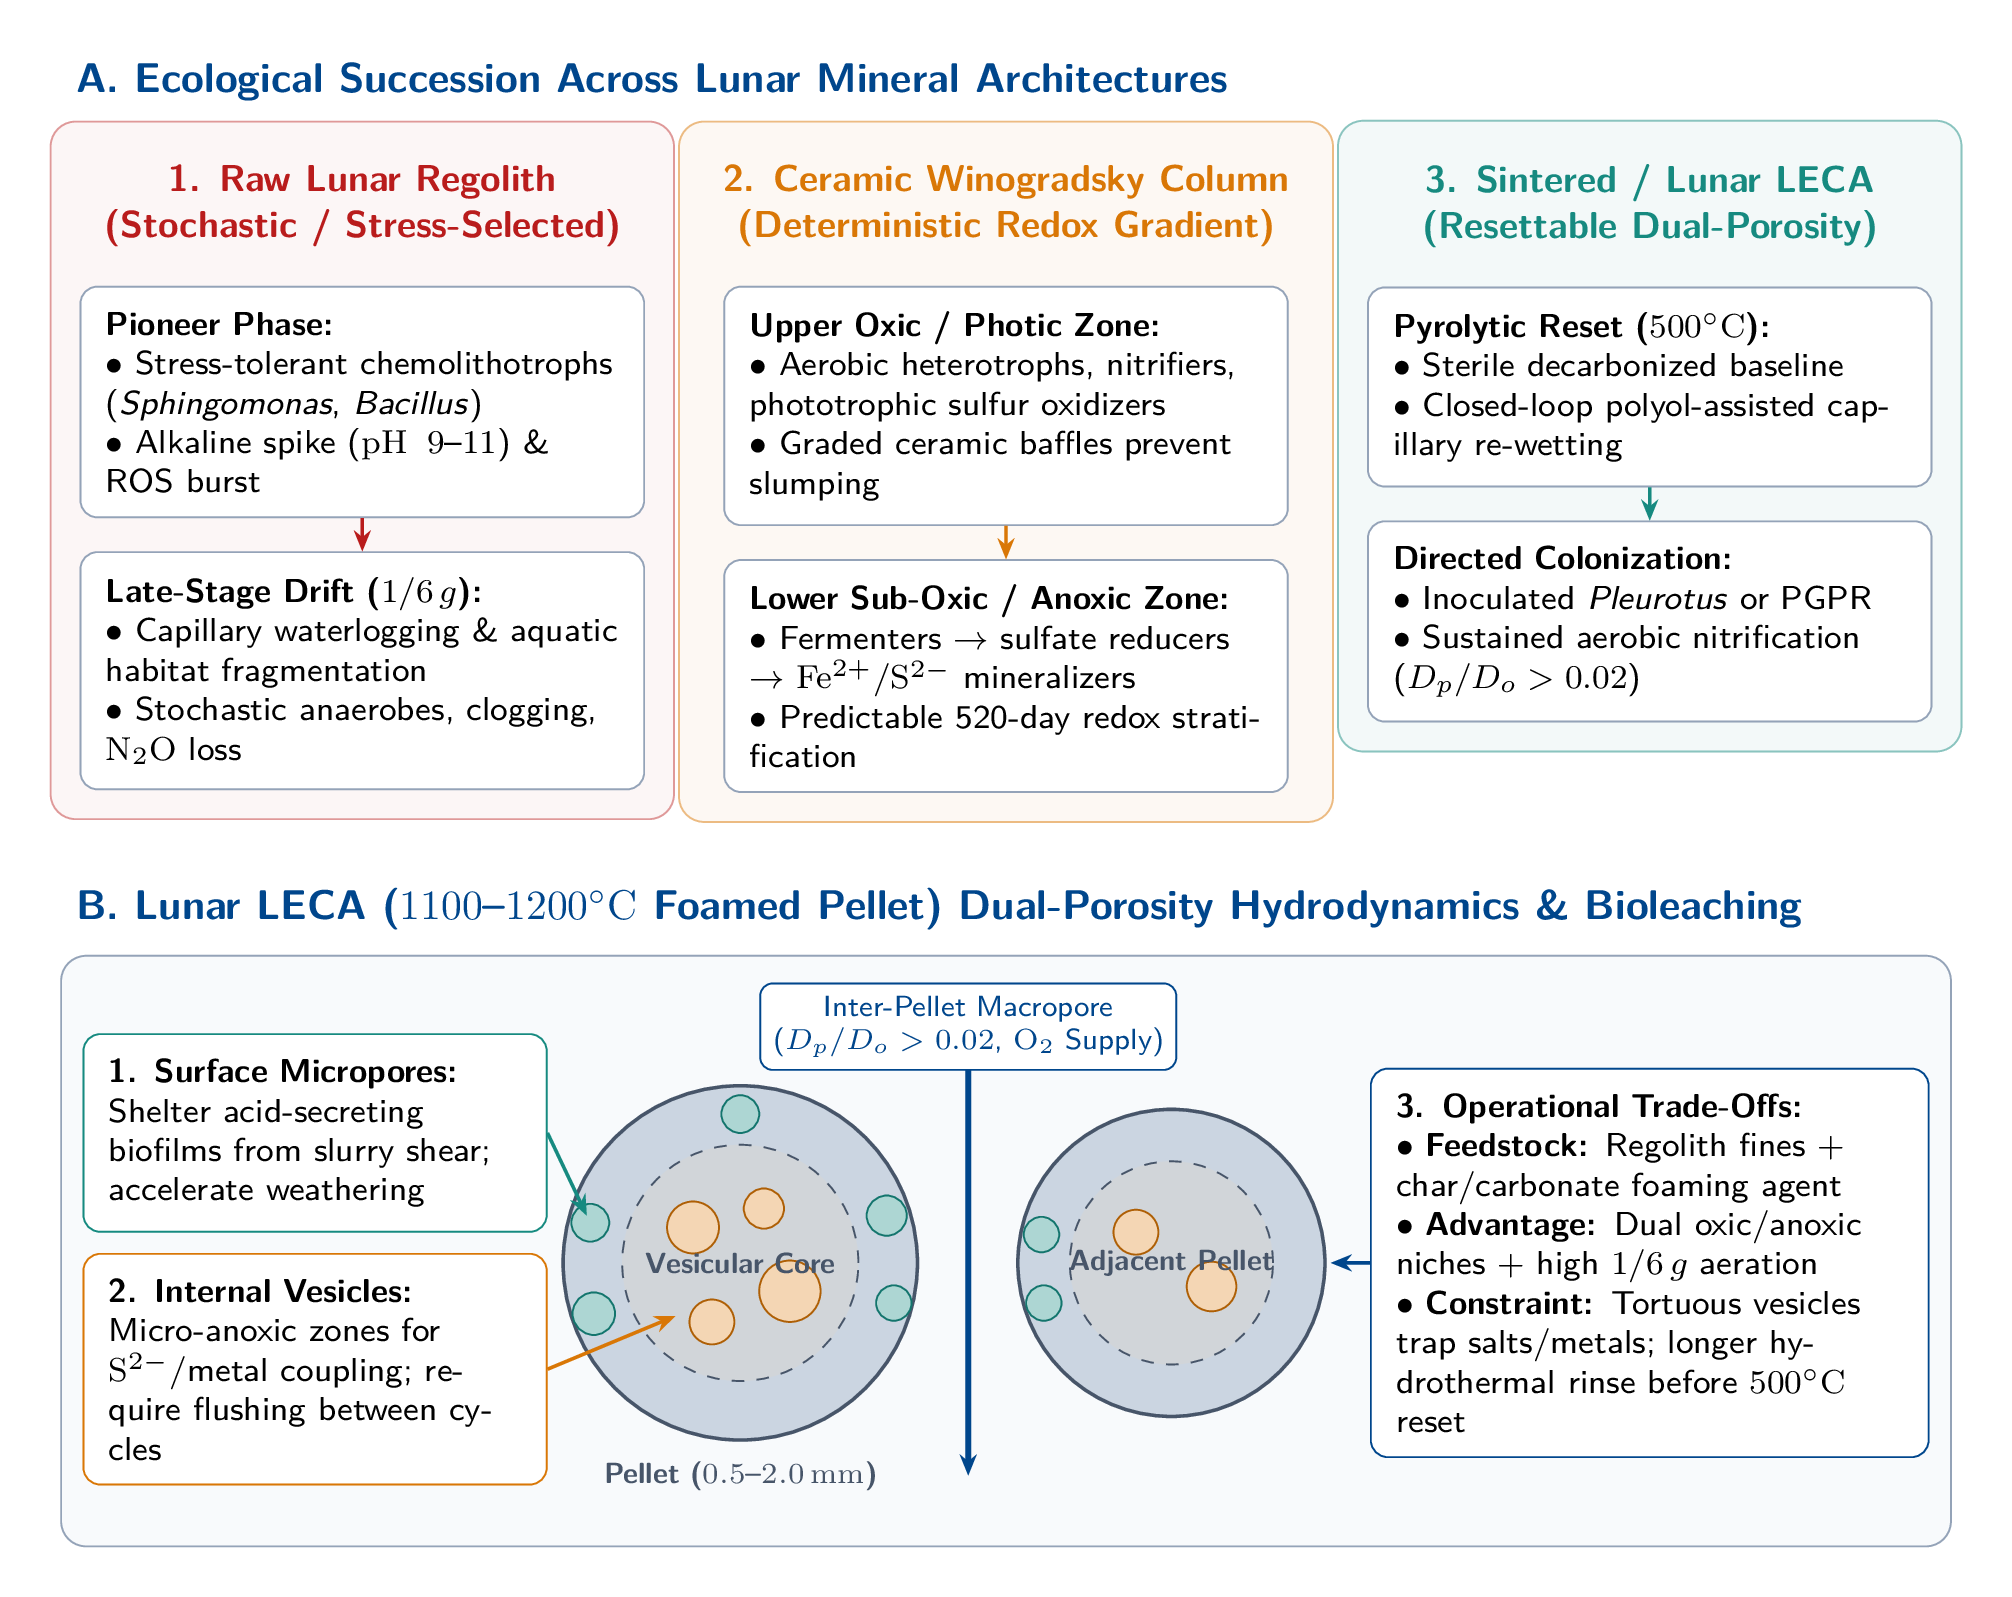
\includegraphics[width=\textwidth]{figures/fig5_microbial_succession_leca.png}
    \caption{\textbf{Microbial succession trajectories and Lunar LECA dual-porosity hydrodynamics.} \textbf{(A)} Ecological succession pathways across raw lunar regolith (stochastic, stress-selected), ceramic Winogradsky columns (deterministic vertical redox stratification), and resettable sintered/Lunar LECA substrates. \textbf{(B)} Conceptual cross-section of foamed Lunar LECA pellets ($0.5\text{--}2.0\,\mathrm{mm}$), illustrating inter-pellet macropores ($D_p/D_o > 0.02$), shear-sheltered surface micropores, and internal micro-anoxic vesicles.}
    \label{fig:microbial_succession_leca}
\end{figure}

\begin{table}[t!]
\centering
\caption{\textbf{Comparative design matrix of engineered lunar ceramic substrate architectures for microbial succession, bioweathering, and cultivation.}}
\label{tab:ceramic_substrate_variants}
\footnotesize
\begin{tabularx}{\textwidth}{>{\raggedright\arraybackslash}p{2.6cm} >{\raggedright\arraybackslash}X >{\raggedright\arraybackslash}X >{\raggedright\arraybackslash}X}
\toprule
\textbf{Property} & \textbf{Monolithic Sintered Ceramic} & \textbf{Ceramic Winogradsky Column} & \textbf{Lunar LECA Pellets (Dual-Porosity)} \\
\midrule
\textbf{Fabrication \& Geometry} & Microwave/solar sintering ($1100\text{--}1200^\circ\mathrm{C}$); rigid blocks, wicking pins, or PWM troughs. & Graded porous ceramic baffles and annular rings sintered inside sealed columns. & Rotary-kiln/microwave firing ($1100\text{--}1200^\circ\mathrm{C}$) with char/carbonate foaming agent; $0.5\text{--}2.0\,\mathrm{mm}$ spheres. \\
\textbf{Pore Architecture} & Unimodal or bimodal capillary channels ($30\text{--}60\,\mu\mathrm{m}$ wicking; $0.5\text{--}2\,\mathrm{mm}$ aeration). & Vertically stratified pore-size gradient enforcing oxygen and redox depth profiles. & Inter-pellet macropores ($0.5\text{--}2\,\mathrm{mm}$) + open surface micropores + closed internal vesicles. \\
\textbf{Microbial Succession} & Resettable via $500^\circ\mathrm{C}$ pyrolysis; favors pioneer PGPR or \textit{Pleurotus} hyphae. & Deterministic 520-day vertical redox succession (aerobes $\to$ $\mathrm{SO}_4^{2-}$ reducers). & Coupled surface-aerobic bioleaching/nitrification and intra-pellet micro-anoxic niches. \\
\textbf{Primary BLSS Role} & Crop root/hyphal support and passive capillary nutrient delivery. & Long-duration regolith bioweathering and biogeochemical metal immobilization. & Fluidized/packed-bed biofiltration, shear-sheltered bioleaching, and lightweight media. \\
\textbf{Regeneration \& Risks} & Rapid $500^\circ\mathrm{C}$ bake-out and ash flush; minimal salt trapping. & Periodic core harvesting; slow turnover if sulfide precipitates clog lower baffles. & Requires extended hydrothermal flushing to clear tortuous vesicles prior to $500^\circ\mathrm{C}$ reset. \\
\bottomrule
\end{tabularx}
\end{table}

\subsection{Thermal Substrate Regeneration and Materials Upcycling}
\label{subsec:thermal_regeneration}

Over continuous cultivation cycles, hydroponic substrates accumulate senescent root fragments, organic root exudates, and microbial biofilms\cite{ming1989lunar}. In terrestrial greenhouse operations, organic fouling clogs pore networks and harbors phytopathogens, necessitating the disposal and replacement of substrates such as rockwool\cite{ming1989lunar,wamelink2019crop}. Sintered ceramics, by contrast, possess the thermal durability required for cyclic regeneration\cite{ming1989lunar,barta1994thermal}.

Following harvest, root-bound ceramic modules undergo pyrolytic oxidation at $500^\circ\mathrm{C}$ in a controlled oxygen atmosphere\cite{ming1989lunar,barta1994thermal}. At this temperature, the aluminosilicate ceramic substrate remains dimensionally and microstructurally stable, whereas all accumulated organic root biomass, extracellular polysaccharides, and biofilms are pyrolyzed and oxidized\cite{ming1989lunar,barta1994thermal}:
\begin{equation}
    \mathrm{C}_x\mathrm{H}_y\mathrm{O}_z (\text{biomass}) + \left(x + \frac{y}{4} - \frac{z}{2}\right)\mathrm{O}_2 \xrightarrow{500^\circ\mathrm{C}} x\,\mathrm{CO}_2 + \frac{y}{2}\,\mathrm{H}_2\mathrm{O} + \text{Mineral Ash}
    \label{eq:pyrolytic_bakeout}
\end{equation}

The volatilized carbon dioxide and water vapor are directed into the habitat ECLSS loop; moisture is recovered via condensing heat exchangers, while $\mathrm{CO}_2$ is returned to the crop canopy for photosynthesis\cite{wheeler2017agriculture,ming1989lunar,barta1994thermal}. The residual mineral ash, containing non-volatile potassium, phosphorus, and trace nutrients, is washed out and redissolved into the liquid fertilizer inventory\cite{ming1989lunar,hendrix2019measurement}. The ceramic matrix emerges sterile, decarbonized, and with unclogged pore channels, ready for immediate replanting without structural degradation\cite{ming1989lunar}.

Crucially, empirical lunar-gravity fluid dynamics indicate that re-wetting high-temperature baked porous substrates against fractional gravity can encounter initial wetting resistance or boundary contact-angle pinning\cite{hasenstein2026assessing}. Hasenstein et al. demonstrated that dilute glycerol solutions dramatically enhance boundary wetting under simulated lunar gravity ($1.76\,\mathrm{m/s}^2$), increasing effective capillary length from $4.2\,\mathrm{mm}$ to $5.2\,\mathrm{mm}$ and overcoming microscale wall roughness\cite{hasenstein2026assessing}. Within our closed-loop architecture, biocompatible polyols such as glycerol and mannitol are naturally synthesized as metabolic byproducts during fungal lignocellulose digestion (\textit{Pleurotus} hyphal metabolism) and cyanobacterial cultivation\cite{hasenstein2026assessing,grimm2018mushroom,verseux2022editorial}. Dosing dilute fractions of these internally generated polyols into the re-wetting loop serves as a closed-loop wetting adjuvant, accelerating post-pyrolysis capillary imbibition, preventing dry bypass channels, and imparting osmotic stress protection to newly seeded crops without requiring imported chemical surfactants\cite{hasenstein2026assessing}.

When ceramic modules eventually reach their mechanical fatigue life, they can be crushed and upcycled as LECA-like (Lightweight Expanded Clay Aggregate) hydroponic gravel beds for habitat drainage systems and Winogradsky-style stratified microbial columns, re-ground into raw feedstock for secondary sintering, or utilized as rigid structural scaffolds for mycelium-bound biocomposite construction materials\cite{ming1989lunar,grimm2018mushroom}.

\subsection{Operational Multitrophic Sequencing and Temporal Synchronization}
\label{subsec:operational_sequencing}

Achieving closed-loop operational stability requires tight temporal synchronization between plant physiological lifecycles, microbial bioleaching extraction rates, and rapid pyrolytic substrate regeneration. As demonstrated in the 120-day outpost operational Gantt schedule (Figure~\ref{fig:multitrophic_gantt}), ceramic bio-infrastructure enables continuous nutrient, water, and gas cycling without system downtime:
\begin{itemize}
    \item \textbf{Crop Staggering and Continuous Harvest:} Primary carbohydrate crops such as dwarf wheat (\textit{Triticum aestivum}) follow a 70-day cultivation timeline from capillary imbibition to grain harvest. To provide consistent crew nutrition and avoid surge loads on ECLSS dehumidifiers, salad greens and short-cycle vegetables are grown in staggered 28-to-30-day batches across adjacent vertical modules.
    \item \textbf{Rapid Pyrolytic Substrate Turnaround:} Within 24 hours of wheat harvest (Day 71), root-bound ceramic modules undergo automated $500^\circ\mathrm{C}$ pyrolytic bake-out. Because the inorganic aluminosilicate matrix withstands thermal cycling, all root mass and biofilms are oxidized into recoverable gaseous $\mathrm{CO}_2$ and $\mathrm{H}_2\mathrm{O}$ within hours (Eq.~\ref{eq:pyrolytic_bakeout}). Following a brief mineral ash flush and re-wetting (Days 73--75), the substrate is completely sterile and ready for the next planting cycle on Day 76, eliminating the disposal logistics inherent to disposable hydroponic media.
    \item \textbf{Decoupled Bioweathering Integration:} Operating in an isolated external reactor on a 14-day batch cycle (Days 18--32), microbial bioleaching mobilizes essential cations ($\mathrm{K}^+, \mathrm{Ca}^{2+}, \mathrm{Mg}^{2+}$) and orthophosphate from raw regolith. Tangential ultrafiltration purges bacterial biomass and heavy metals, delivering concentrated ionic replenishment into the primary hydroponic loop on Day 36 to balance nutrient depletion from the maturing crop canopy.
    \item \textbf{Saprotrophic Bioconversion of Inedible Biomass:} Harvested crop straw is milled, steam-pasteurized, and inoculated with \textit{Pleurotus ostreatus} spawn on Day 74. Supported by porous ceramic trays, fungal hyphae colonize the matrix over 14 days, yielding protein-dense fruiting flushes between Days 91 and 98 while respiring metabolic $\mathrm{CO}_2$ directly back into the vegetative wheat chamber.
\end{itemize}

\begin{figure}[t!]
    \centering
    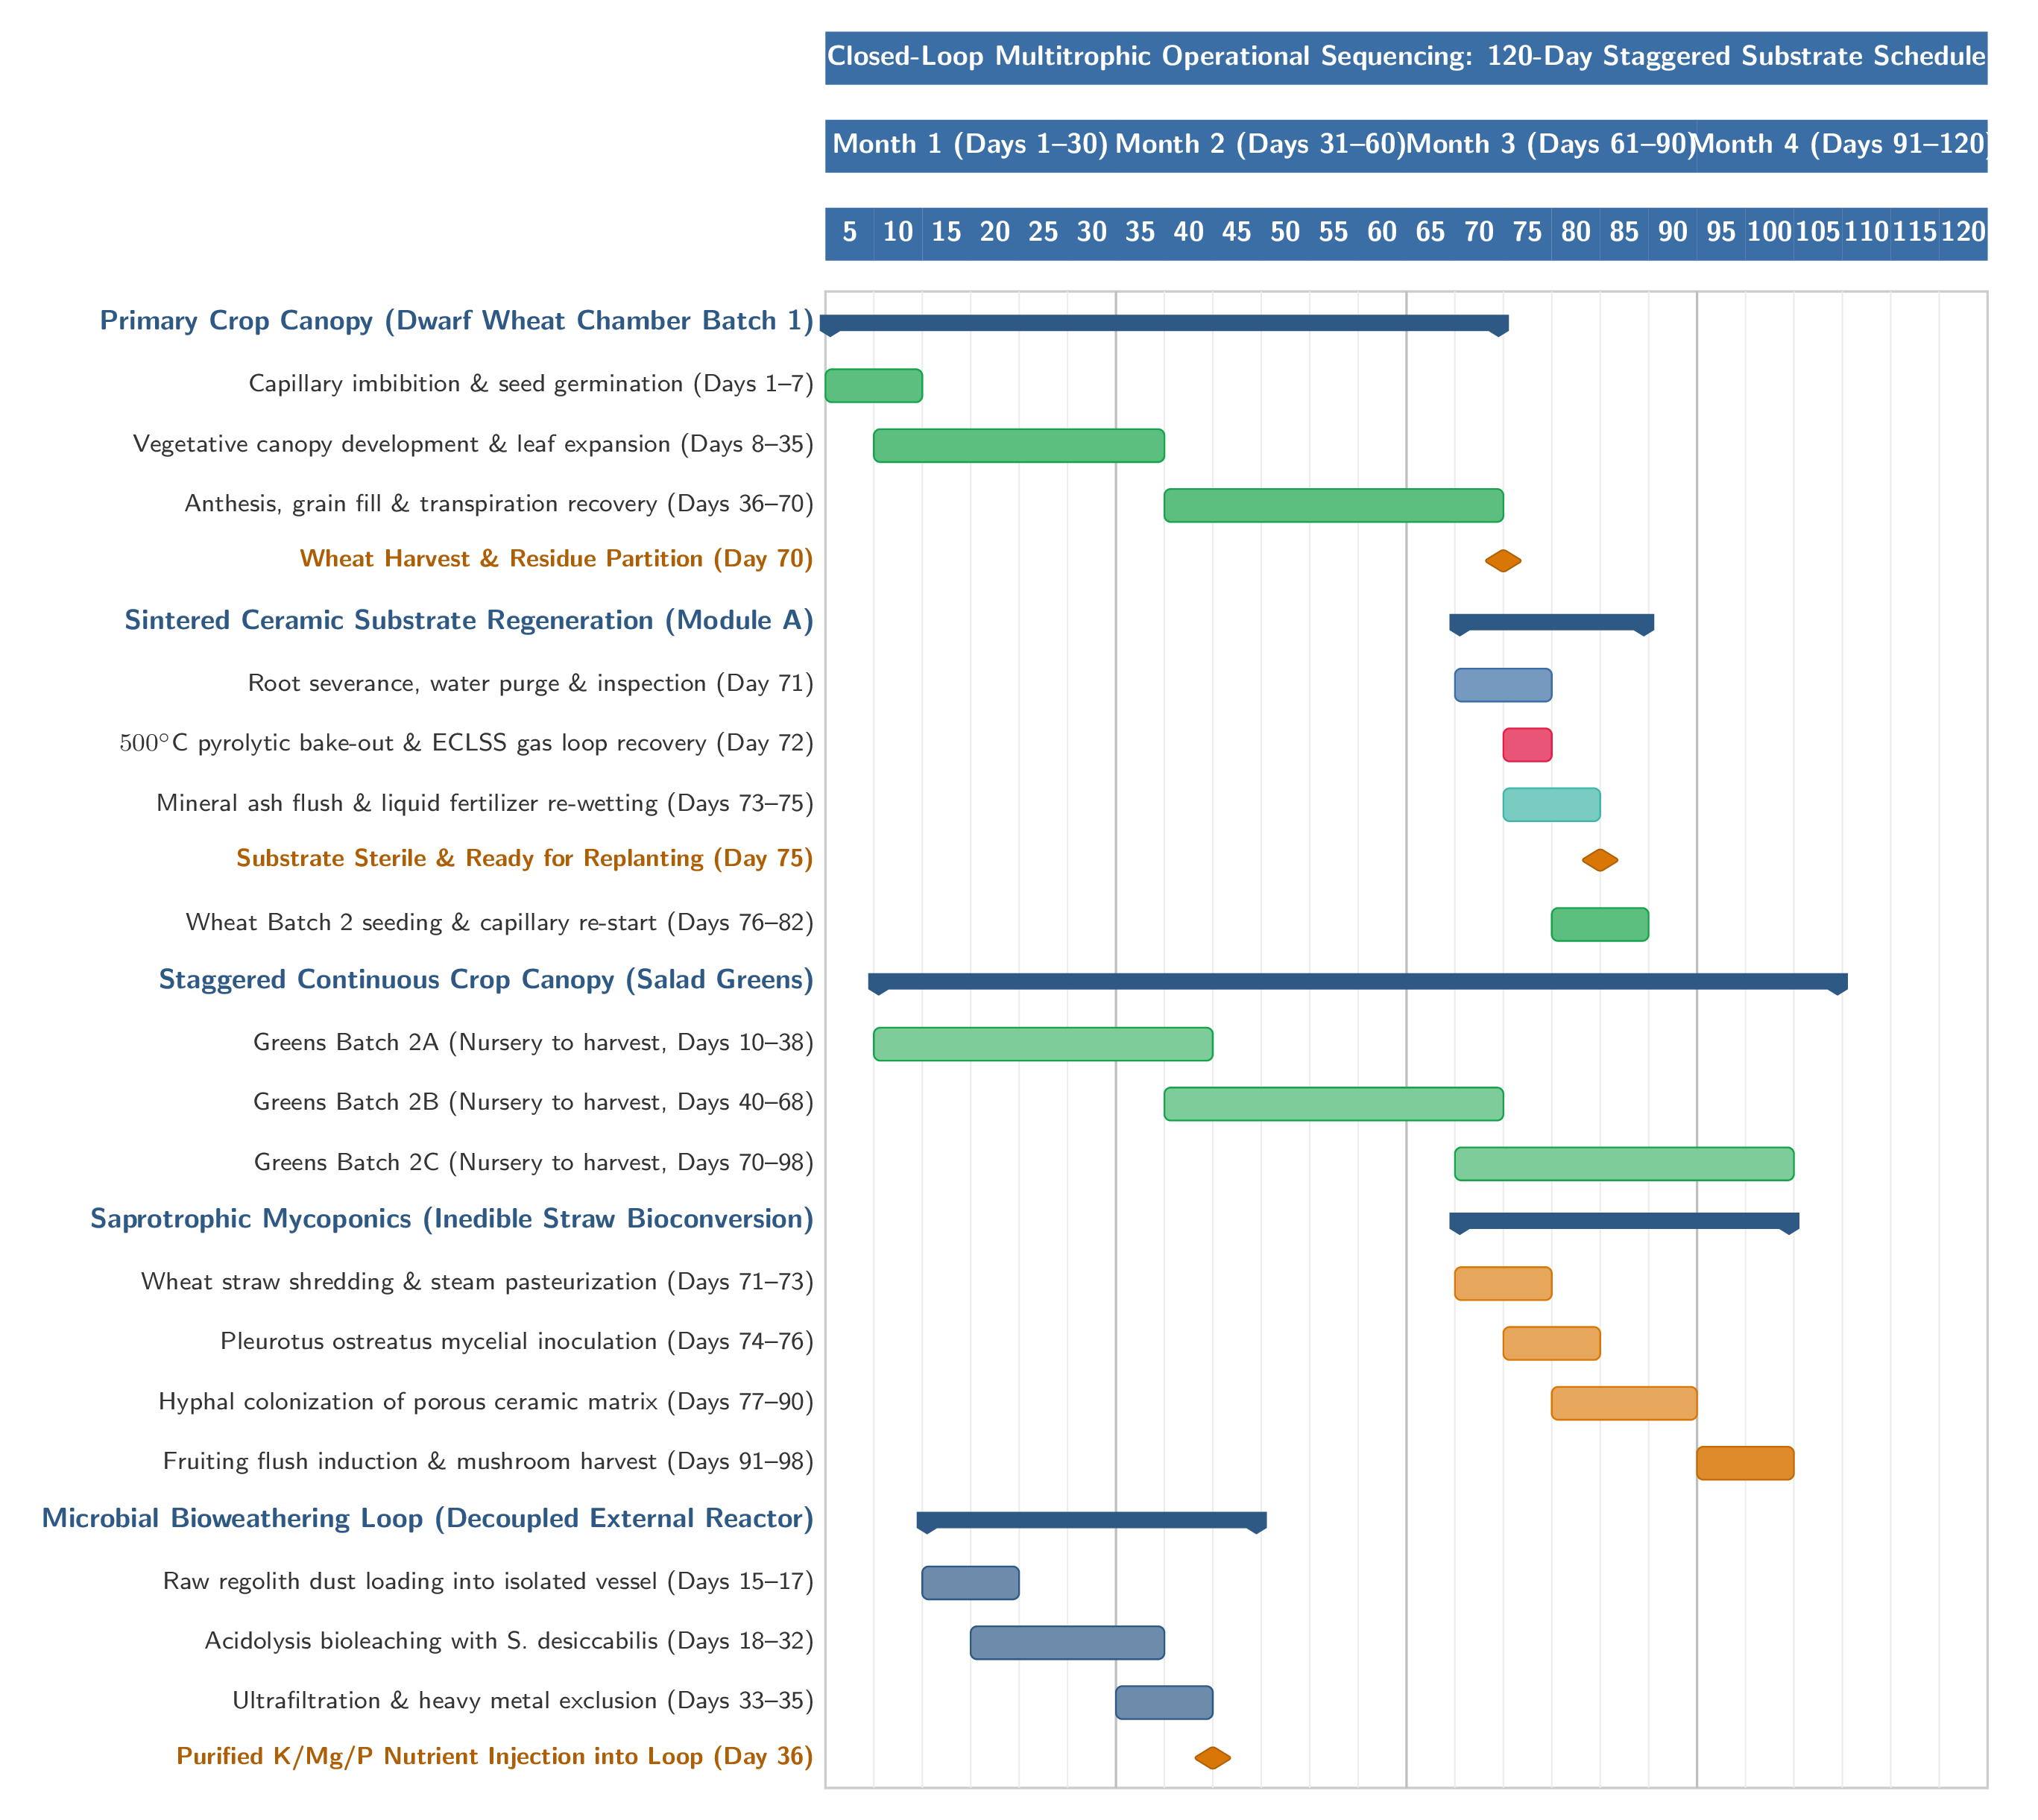
\includegraphics[width=\textwidth]{figures/fig8_multitrophic_gantt.png}
    \caption{\textbf{Closed-loop multitrophic operational sequencing and substrate lifecycle schedule.} A 120-day repeatable outpost schedule illustrating the temporal coordination between dwarf wheat cultivation (70 days), rapid ceramic substrate pyrolytic regeneration at $500^\circ\mathrm{C}$ with closed-loop $\mathrm{CO}_2$/moisture recovery (Days 71--75), staggered salad greens production, saprotrophic mushroom (\textit{Pleurotus ostreatus}) bioconversion of inedible straw (Days 71--98), and external microbial bioweathering cycles providing continuous elemental replenishment with zero agricultural downtime.}
    \label{fig:multitrophic_gantt}
\end{figure}

\section{Strategic Outlook and Technology Development Roadmap}
\label{sec:roadmap}

Transitioning sintered regolith bio-infrastructure from terrestrial laboratory validation to operational lunar deployment requires a structured Technology Readiness Level (TRL) maturation strategy\cite{ming1989lunar,fateri2019solar,santomartino2023toward}. Current research resides predominantly at TRL 2 to 3, characterized by benchtop sintering of lunar regolith simulants and biological assays on returned Apollo samples\cite{paul2022plants,fateri2019solar}. Maturing these technologies into flight-ready systems requires a synchronized, multi-track development roadmap aligned with international Artemis and lunar exploration campaigns (Figures~\ref{fig:trl_roadmap}--\ref{fig:trl_gantt} and Table~\ref{tab:trl_roadmap}):

\begin{figure}[t!]
    \centering
    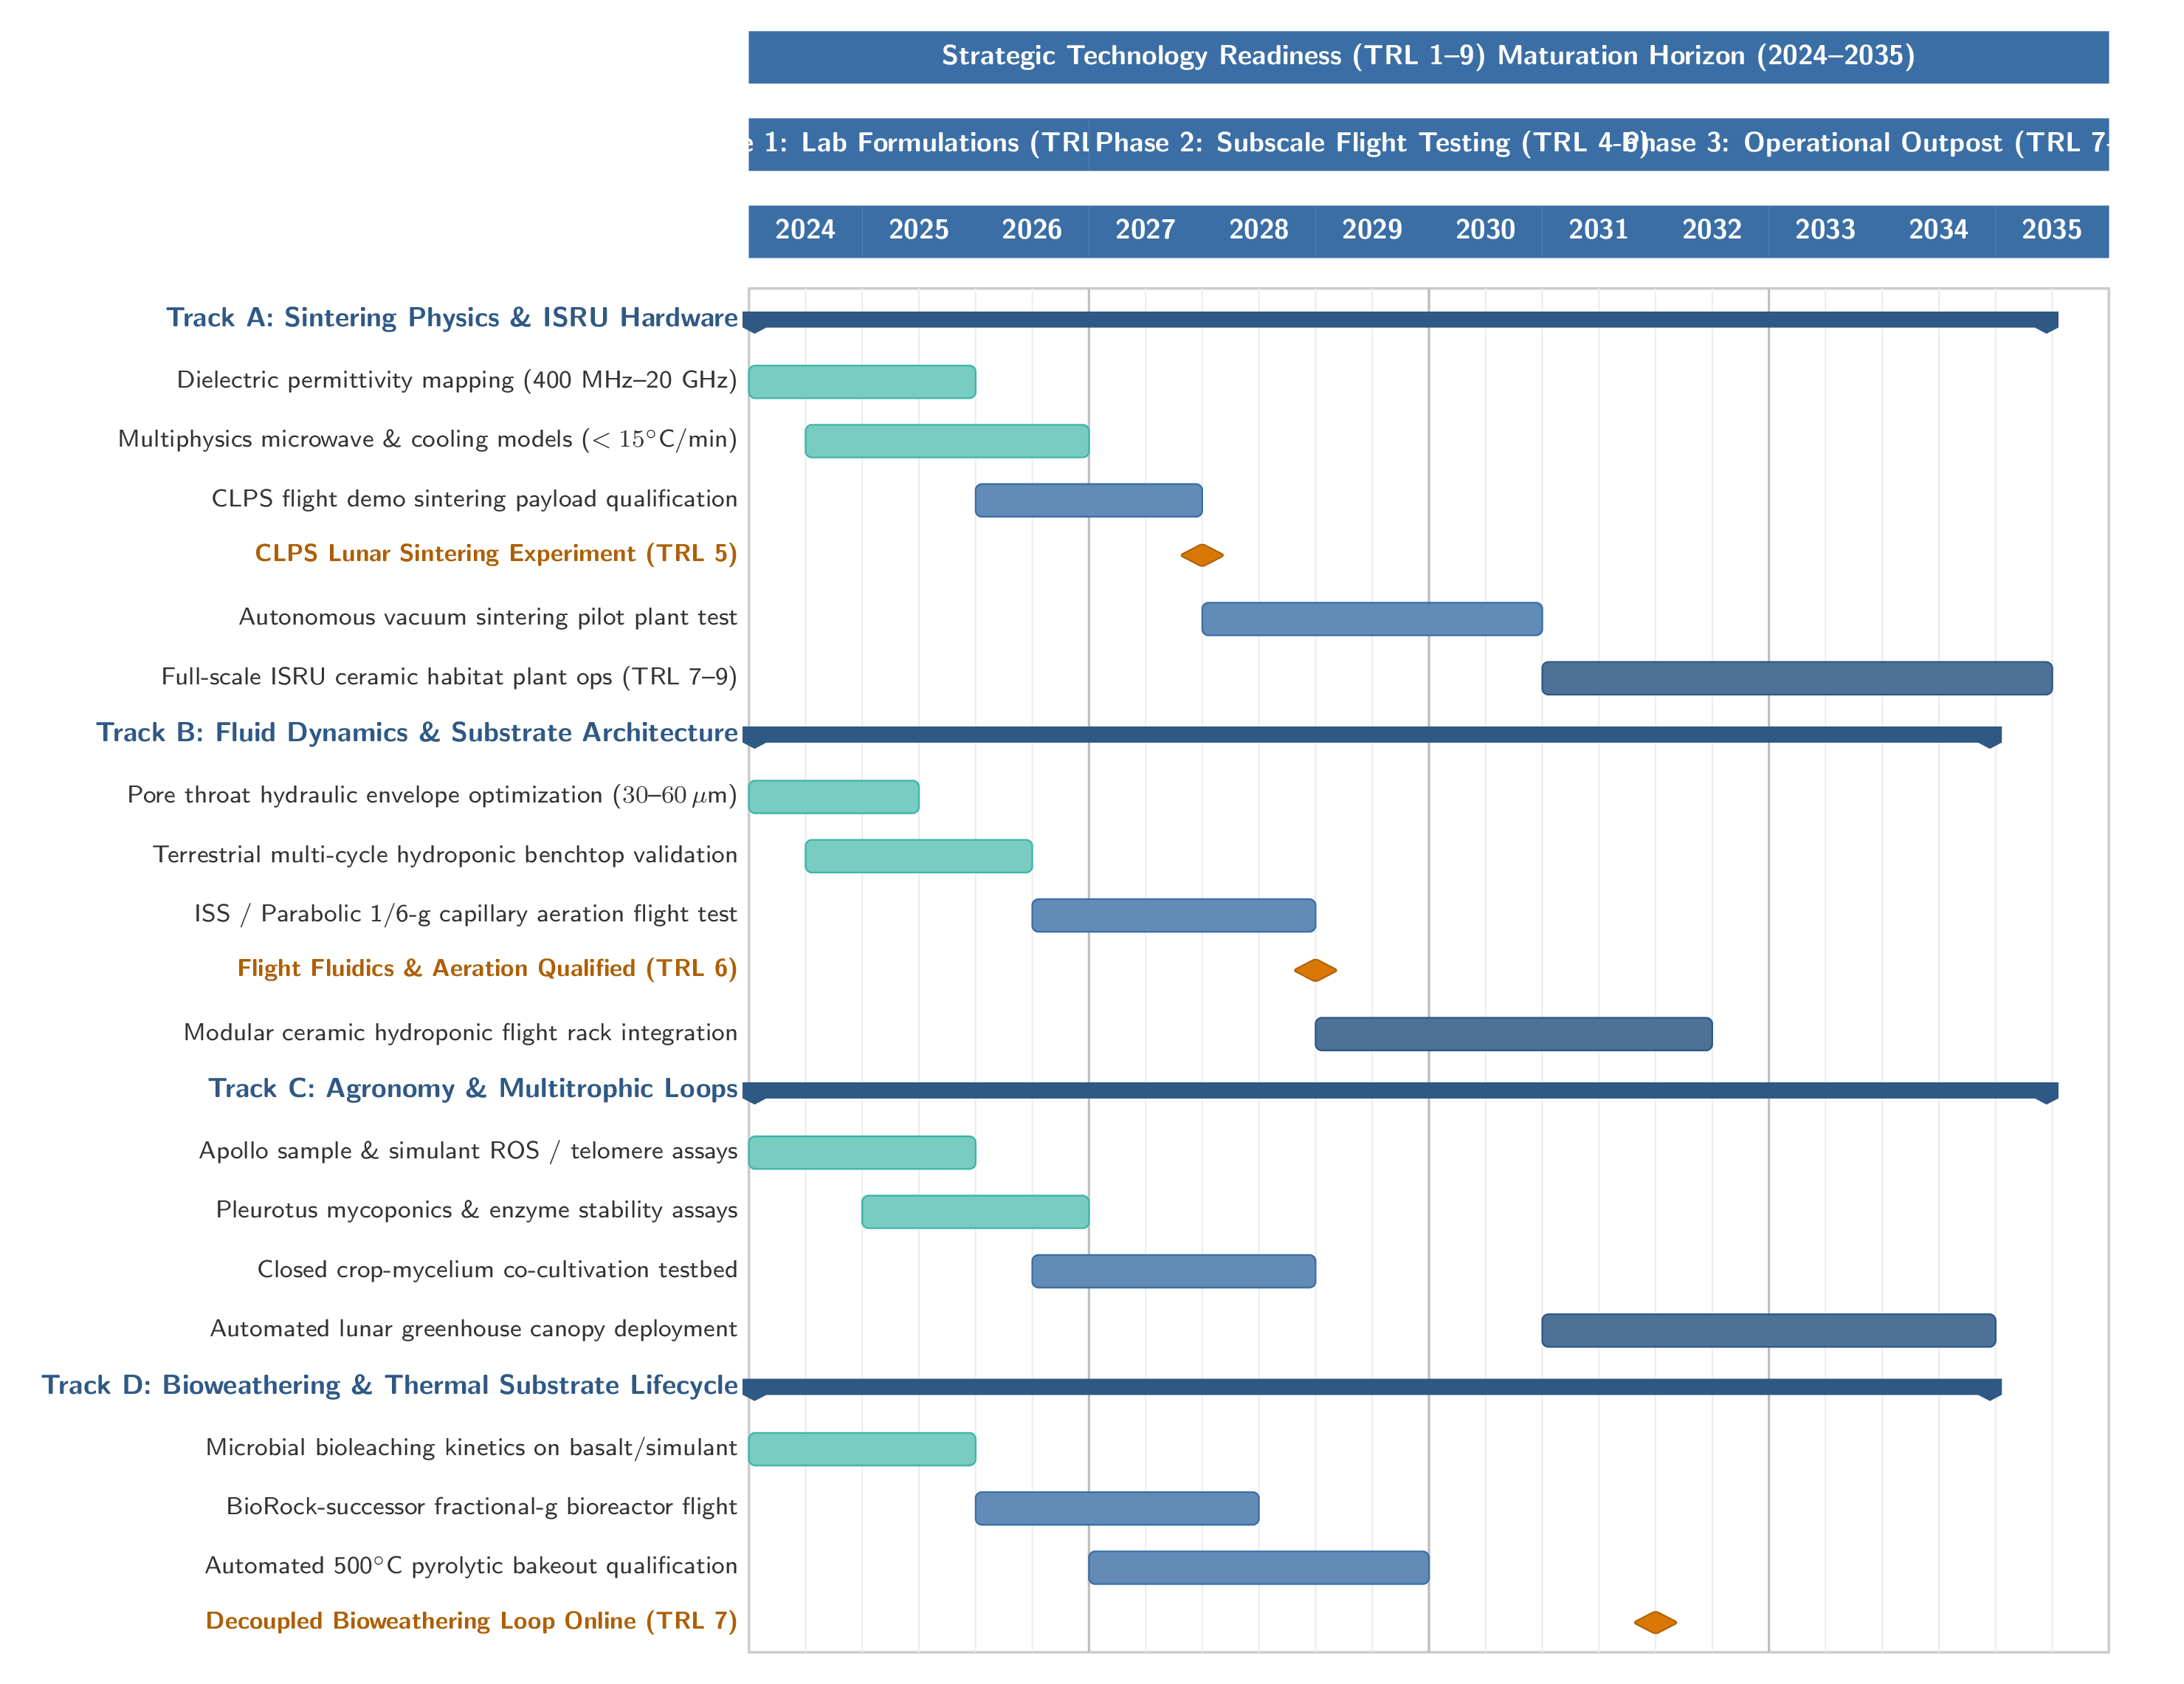
\includegraphics[width=\textwidth]{figures/fig7_trl_gantt.png}
    \caption{\textbf{Strategic technology maturation and multi-track development Gantt schedule (2024--2035).} Concurrent maturation trajectories across Track A (Sintering Physics \& ISRU Hardware), Track B (Fluid Dynamics \& Substrate Architecture), Track C (Agronomy \& Multitrophic Loops), and Track D (Bioweathering \& Substrate Lifecycle). Critical path milestones include the CLPS lunar surface sintering experiment (late 2027), ISS $1/6\,g$ fluidics and aeration qualification (mid 2028), and full-scale habitat ECLSS loop integration ($>$2031).}
    \label{fig:trl_gantt}
\end{figure}

\subsection{Phase 1: Laboratory Formulations and Simulant Validation (2024--2026, \texorpdfstring{TRL 1 $\to$ 3}{TRL 1-3})}
The foundational phase centers on materials characterization and multiphysics process modeling using high-fidelity lunar highland and mare simulants\cite{paul2022plants,ramossomolinos2024electromagnetic}. Key engineering milestones include mapping complex permittivity and dielectric loss tangents across microwave frequencies ($400\,\mathrm{MHz}\text{--}20\,\mathrm{GHz}$)\cite{ramossomolinos2024electromagnetic}, optimizing volumetric electromagnetic coupling\cite{lim2019numerical}, and establishing precise cooling curves ($<15^\circ\mathrm{C/min}$) to eliminate thermal-stress-induced microcracking\cite{xi2026multiphysics}. In parallel, multi-generational botanical and fungal assays must verify that sintered porous substrates fully eliminate the transcriptomic stress, ROS bursts, and telomeric DNA lesions observed in raw regolith\cite{paul2022plants,ming1989lunar,barbero2024telomere}.

\subsection{Phase 2: Subscale Flight Testing and In-Situ Demonstrations (2027--2030, \texorpdfstring{TRL 4 $\to$ 6}{TRL 4-6})}
The demonstration phase advances autonomous hardware to relevant spaceflight environments\cite{ming1989lunar,liu2013microwave,cockell2018biorock}. The foundation for fractional-gravity fluid mechanics has achieved TRL 4 through suborbital flight testing aboard Blue Origin NS-29, which quantified centrifugal lunar-gravity ($1.76\,\mathrm{m/s}^2$) meniscus dynamics, boundary film thickening, and polyol wetting facilitation\cite{hasenstein2026assessing}. Building on this empirical baseline, flight experiments aboard the International Space Station or orbital variable-gravity centrifuges will evaluate two-phase fluid wicking, liquid-gas exchange, and root aeration specifically within sintered regolith ceramic cores under simulated $1/6\,g$, advancing the engineered pore throat envelope ($30\text{--}60\,\mu\mathrm{m}$) to TRL 5--6\cite{ming1989lunar,heinse2007porous,hasenstein2026assessing}. Concurrently, miniaturized microwave and concentrated solar sintering payloads deployed via Commercial Lunar Payload Services (CLPS) landers will validate vacuum degassing, sintering kinetics, and thermal consolidation directly on the lunar surface\cite{ming1989lunar,hendrix2024reactivity,fateri2019solar}. Automated bioreactor payloads will establish continuous microbial bioleaching kinetics from basaltic minerals under fractional gravity\cite{cockell2018biorock,santomartino2023toward,cockell2020microbially}.

\subsection{Phase 3: Operational Habitat Integration and Autonomous Production (\texorpdfstring{$>$2031}{>2031}, \texorpdfstring{TRL 7 $\to$ 9}{TRL 7-9})}
The operational phase achieves full integration within a permanent lunar surface base\cite{ming1989lunar,metzger2023cost,anderson2021lunar}. Automated ISRU manufacturing systems will excavate and classify raw regolith, sinter modular hydroponic troughs, and install them into habitat life-support racks\cite{ming1989lunar,fateri2019solar,metzger2023cost}. The agricultural architecture will connect photoautotrophic crop canopies, saprotrophic mushroom cultivation, and external microbial bioweathering reactors into an interconnected closed loop\cite{ming1989lunar,grimm2018mushroom,verseux2022editorial,cockell2018biorock}. Incorporating automated $500^\circ\mathrm{C}$ pyrolytic bake-out cycles will enable infinite substrate re-use and $>98.5\%$ water recovery, providing a durable foundation for long-duration human life support on the lunar surface\cite{ming1989lunar,anderson2021lunar,barta1994thermal}.

\subsection{Concurrent Multi-Track Maturation and Critical Path Dependencies}
As mapped in the strategic Gantt schedule (Figure~\ref{fig:trl_gantt}), advancing lunar bio-infrastructure requires de-risking four concurrent technical tracks rather than pursuing sequential milestones:
\begin{itemize}
    \item \textbf{Track A (Sintering Physics \& ISRU):} Precursor materials characterization and multiphysics simulations directly inform the flight payload design scheduled for CLPS surface validation by late 2027 (TRL 5). Surface qualification under hard vacuum ($10^{-10}\,\mathrm{Torr}$) provides the empirical thermal constants necessary to scale the autonomous pilot plant to operational status (TRL 7--9) by 2031.
    \item \textbf{Track B (Multiphase Fluid Dynamics):} Suborbital flight validation aboard Blue Origin NS-29 established TRL 4 proof-of-concept for lunar-g fluid mechanics\cite{hasenstein2026assessing}, complemented by NASA's ISS Plant Water Management (PWM-5/6, PSI-187) passive capillary fluidics datasets\cite{weislogel2026pwm,hatch2022pwm,pwm2020ntrs} and variable-gravity vadose transport models\cite{jones2012beyond}. Follow-on flight experiments on ISS variable-gravity centrifuges or parabolic platforms (2026--2028) will evaluate continuous nutrient wicking, bubble management, and zero-hypoxia aeration through sintered ceramic cores (TRL 5--6), ensuring hydraulic stability before modular hydroponic racks are integrated into habitat structures.
    \item \textbf{Track C (Crop Canopy \& Multitrophic Loops):} Early botanical transcriptomic assays (TRL 1--3) transition into co-cultivation testbeds linking crops and saprotrophic fungi, establishing the baseline yield models required for habitat life-support sizing.
    \item \textbf{Track D (Bioweathering \& Substrate Lifecycle):} Terrestrial microbial leaching kinetics transition into microgravity bioreactor demonstrations (building on the ESA BioRock legacy), ensuring continuous in-situ fertilizer replenishment is fully decoupled from the active plant root zone before full-scale base commissioning.
\end{itemize}

\subsection{Microbial and Fungal Integration Across the Lunar BLSS Narrative}
\label{subsec:microbial_fungal_roadmap}

While engineering controls passivate abiotic regolith hazards and stabilize $1/6\,g$ root-zone hydrodynamics, long-duration crop productivity ultimately depends on intentional cross-kingdom management of bacteria and fungi\cite{sikes2026charting}. As synthesized by Sikes et al. (2026), keeping plants sterile during crewed missions is infeasible; initially sterile substrates act as undirected assembly experiments in which \textbf{community coalescence} with crew-associated Microbiome of the Built Environment (MoBE) taxa, air/water-line biofilms, and antimicrobial resistance (AMR) reservoirs can trigger opportunistic disease---exemplified by the \textit{Fusarium oxysporum} outbreak on \textit{Zinnia hybrida} in the ISS VEGGIE facility\cite{sikes2026charting,schuerger2021fusarium,baxter2026biofilms}. Integrating defined microbial and fungal partners directly strengthens each core narrative of this roadmap (Table~\ref{tab:microbial_fungal_integration}):
\begin{itemize}
    \item \textbf{Toxicology \& Model-to-Crop Translation (Section~\ref{sec:toxicology}):} Sikes et al. (2026) highlight that \textit{Arabidopsis thaliana} cannot form symbioses with arbuscular mycorrhizal (AM) fungi or nitrogen-fixing rhizobia and differs from monocot cereals in salicylic acid immune signaling\cite{sikes2026charting}. Phase 1 validation must therefore expand to \textit{Medicago truncatula} (rhizobia/AM models) and \textit{Brachypodium distachyon} (cereal-fungal pathosystems), pairing sintered ceramic passivation with AM fungi and ROS-alleviating endophytes that remediate residual regolith stress and enable seed-to-seed completion\cite{sikes2026charting,atkin2026bioremediation}.
    \item \textbf{Substrate Architecture \& Coalescence Control (Sections~\ref{sec:manufacturing}--\ref{sec:fluid_dynamics}):} Because microgravity alters liquid--gas transport and promotes waste-$\mathrm{CO}_2$ bubble accumulation and biofilm clogging\cite{sikes2026charting,baxter2026biofilms}, sintered ceramics with $30\text{--}60\,\mu\mathrm{m}$ wicks and $>0.5\,\mathrm{mm}$ aeration channels ($D_p/D_o > 0.02$) must be paired with ecological priority effects. Following each $500^\circ\mathrm{C}$ pyrolytic bake-out, immediate polyol-assisted re-wetting with defined \textbf{Synthetic Communities (SynComs)} and obligate plant biotrophs occupies rhizosphere niches before opportunistic MoBE pathogens can establish\cite{sikes2026charting}.
    \item \textbf{ESM Economics \& Crop Nutrition (Section~\ref{sec:esm_analysis}):} Microgravity-grown crops frequently exhibit reduced calcium, magnesium, and iron concentrations\cite{sikes2026charting}. Nitrogen-fixing rhizobia, phosphate-solubilizing AM fungi, and endophytic symbionts offset these mineral deficits while reducing external fertilizer and chemical buffer resupply, reinforcing the ESM advantage of sintered ceramic architectures\cite{sikes2026charting,atkin2026bioremediation}.
    \item \textbf{Closed-Loop Multitrophic Coupling (Section~\ref{sec:closed_loop}):} Beyond edible crops, saprotrophic fungi (\textit{Pleurotus ostreatus}), Winogradsky/Lunar LECA bioleaching consortia, and non-food phytoremediating/lignocellulosic crops (e.g., willow, hemp) rely on rhizosphere bacteria and fungi to convert inedible straw and leachates into protein, polyols, and purified mineral permeate\cite{sikes2026charting,cockell2018biorock,babcsanyi2017biogeochemical}.
    \item \textbf{Assembly-First Multiomics \& Biobanking Gateways (TRL 1 $\to$ 9):} To verify that mutualisms remain stable under partial gravity and radiation, Sikes et al. (2026) recommend replacing poly(A)-biased single-omics with \textbf{assembly-first multiomics}---combining de novo whole-metagenome co-assembly, non-poly(A)-biased metatranscriptomics, and untargeted metabolomics alongside standardized NASA NBISC/OSDR archiving across Phases 1--3\cite{sikes2026charting}.
\end{itemize}

\begin{table}[t!]
\centering
\caption{\textbf{Cross-narrative integration of microbial and fungal guilds into the lunar sintered regolith BLSS roadmap (aligned with Sikes et al., 2026\cite{sikes2026charting}).}}
\label{tab:microbial_fungal_integration}
\footnotesize
\begin{tabularx}{\textwidth}{>{\raggedright\arraybackslash}p{2.5cm} >{\raggedright\arraybackslash}X >{\raggedright\arraybackslash}X >{\raggedright\arraybackslash}X}
\toprule
\textbf{Manuscript Narrative} & \textbf{Target Microbial / Fungal Guilds} & \textbf{Spaceflight Risk Mitigated} & \textbf{TRL Integration Milestone} \\
\midrule
Toxicology \& Mineral Passivation & AM fungi, ROS-alleviating endophytes, \textit{Medicago} / \textit{Brachypodium} models & Residual metal/ROS stress; \textit{Arabidopsis} non-mycorrhizal bias & Phase 1 (TRL 2--3): Seed-to-seed AM/SynCom trials on sintered ceramics\cite{atkin2026bioremediation,sikes2026charting} \\
Substrates \& $1/6\,g$ Fluidics & Defined SynComs, obligate plant biotrophs, nitrifying biofilms & Uncontrolled MoBE coalescence, AMR, \textit{Fusarium} outbreaks, biofilm hypoxia\cite{schuerger2021fusarium,baxter2026biofilms} & Phase 2 (TRL 4--6): Post-pyrolysis SynCom inoculation in $1/6\,g$ wicks/PWM troughs \\
ESM \& Crop Nutrition & Rhizobia ($\mathrm{N}_2$ fixation), P-solubilizing AM fungi, PGPR & Ca/Mg/Fe crop deficiencies; chemical buffer \& fertilizer resupply mass & Phase 2--3 (TRL 5--8): Quantify fertilizer ESM offset in flight testbeds \\
Closed-Loop Ecosystems & \textit{Pleurotus} saprotrophs, \textit{Sphingomonas}/\textit{Bacillus} bioleachers, Winogradsky consortia & Inedible straw accumulation, heavy-metal co-leaching, $\mathrm{N}_2\mathrm{O}$ loss & Phase 3 (TRL 7--9): Coupled mycoponics, Lunar LECA biofilters, \& $500^\circ\mathrm{C}$ reset \\
Multiomics Verification & Whole rhizosphere/endosphere \& MoBE source tracking & Poly(A) bacterial RNA loss; low-abundance signal filtering & Phases 1--3: De novo WMS co-assembly, untargeted metabolomics, NBISC archiving\cite{sikes2026charting} \\
\bottomrule
\end{tabularx}
\end{table}

\begin{figure}[t!]
    \centering
    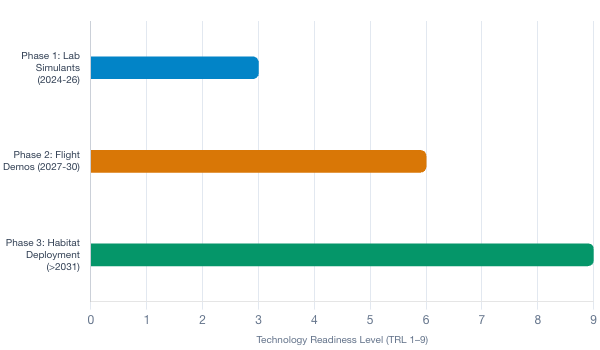
\includegraphics[width=0.85\textwidth]{figures/fig6_trl_roadmap.png}
    \caption{\textbf{Technology Readiness Level (TRL 1--9) maturation horizon for lunar sintered regolith bio-infrastructure.} Strategic progression from Phase 1 laboratory formulations (TRL 1--3, 2024--2026), through Phase 2 subscale flight demonstrations on CLPS landers and the ISS (TRL 4--6, 2027--2030), to Phase 3 operational ISRU habitat integration and closed-loop ECLSS deployment ($>$2031, TRL 7--9).}
    \label{fig:trl_roadmap}
\end{figure}

\begin{table}[t!]
\small
\centering
\caption{\textbf{Strategic technology maturation roadmap for sintered regolith bio-infrastructure.}}
\label{tab:trl_roadmap}
\begin{tabularx}{\textwidth}{lcXX}
\toprule
\textbf{Maturation Phase} & \textbf{Target TRL} & \textbf{Key Technical Milestones} & \textbf{Primary Risks \& Engineering Mitigations} \\
\midrule
Phase 1: Laboratory Formulations (2024--2026) & TRL $1 \to 3$ & Measure dielectric loss tangents across simulants; validate coupled multiphysics models; verify chemical passivation of $\mathrm{npFe}^0$\cite{ming1989lunar,xi2026multiphysics,ramossomolinos2024electromagnetic}. & \textbf{Risk:} Thermal shock cracking during cooling.\newline \textbf{Mitigation:} Enforce controlled cooling rates $<15^\circ\mathrm{C/min}$\cite{xi2026multiphysics}. \\
\addlinespace
Phase 2: Subscale Flight Testing (2027--2030) & TRL $4 \to 6$ & Leverage NS-29 suborbital lunar-g fluidics baseline (TRL 4)\cite{hasenstein2026assessing}; deploy autonomous sintering payloads on CLPS landers; validate $1/6\,g$ wicking in sintered cores on ISS\cite{ming1989lunar,fateri2019solar,heinse2007porous,hasenstein2026assessing}. & \textbf{Risk:} Multiphase fluid separation failure under $1/6\,g$.\newline \textbf{Mitigation:} Constrain pore throat diameters to $30\text{--}60\,\mu\mathrm{m}$\cite{ming1989lunar}. \\
\addlinespace
Phase 3: Operational Deployment ($>2031$) & TRL $7 \to 9$ & Deploy full-scale ISRU manufacturing plant; integrate sintered hydroponics with base ECLSS loops\cite{ming1989lunar,chinnannan2025spirulina,metzger2023cost}. & \textbf{Risk:} Long-term substrate biofouling and pore clogging.\newline \textbf{Mitigation:} Implement cyclic $500^\circ\mathrm{C}$ pyrolytic regeneration\cite{ming1989lunar,santomartino2023toward}. \\
\bottomrule
\end{tabularx}
\end{table}

\section{Conclusions}
\label{sec:conclusions}

Direct edaphic cultivation in raw lunar regolith presents fundamental biological, toxicological, and fluid-mechanical barriers that cannot be resolved through chemical fertilization alone\cite{paul2022plants,ming1989lunar,krejci2026lunar}. Molecular, transcriptomic, and toxicological investigations confirm that pristine lunar dust contains reactive nanophase metallic iron ($\mathrm{npFe}^0$), unpassivated silicate dangling bonds, and razor-sharp mineral shards that trigger chronic oxidative stress cascades, inflict 8-oxoguanine genomic lesions, accelerate telomere shortening, and arrest plant root development\cite{paul2022plants,ming1989lunar,hendrix2024reactivity,barbero2024telomere}. Simultaneously, the reduction of gravitational acceleration to $1/6\,g$ lowers the Bond number and establishes a capillary-dominated hydraulic regime, with empirical flight data from Blue Origin NS-29 demonstrating suppressed capillary length ($L_c \approx 4.2\,\mathrm{mm}$) and boundary film thickening\cite{hasenstein2026assessing}. Coupled with intrinsic particle hydrophobicity (confirmed on Chang'e-5 samples\cite{zhang2025wettability}) and the absence of coarse aerating fractions in surface dust without multi-meter excavation\cite{mckay1991lunar,zhao2023variations,hasenstein2026assessing}, polydisperse regolith beds inevitably suffer severe capillary waterlogging, dry bypass channeling, and root-zone hypoxia\cite{ming1989lunar,ostrach1982low,hasenstein2026assessing,stout2001evidence}.

Transforming in-situ regolith into engineered sintered ceramics offers an ISRU manufacturing paradigm that fundamentally circumvents these edaphic constraints\cite{ming1989lunar,taylor2005microwave}. Thermal processing above $1050^\circ\mathrm{C}$ passivates reactive geochemical interfaces by solid-solubilizing $\mathrm{npFe}^0$ into stable augite and olivine crystal frameworks, rounds abrasive grain edges, and quenches dangling surface radicals, creating an inert, biocompatible growth substrate\cite{ming1989lunar,hendrix2019measurement,xi2026multiphysics}. Pre-sintering classification of regolith particles to $45\text{--}75\,\mu\mathrm{m}$ produces monodisperse pore throat diameters of $30\text{--}60\,\mu\mathrm{m}$, stabilizing matric potential within the optimal window ($-2.5$ to $-5.0\,\mathrm{kPa}$) while maintaining air-filled porosity above $25\text{--}30\%$ for unhindered aerobic root respiration under fractional gravity\cite{ming1989lunar,heinse2007porous}.

From a mission systems perspective, the upfront launch mass required for an autonomous sintering plant is offset rapidly by operational efficiencies\cite{ming1989lunar,hanford2004advanced,metzger2023cost}. Life cycle assessments based on NASA Equivalent System Mass formulations demonstrate an operational breakeven horizon between $18$ and $22$ months compared to direct regolith cultivation (and as low as $9\text{--}15$ months under surface nuclear power architectures)\cite{ming1989lunar,chinnannan2025spirulina,colozza2020power}. This advantage is driven by $>98.5\%$ water recovery efficiency, intrinsic $\mathrm{pH}$ stability, and the elimination of chemical buffer resupply\cite{ming1989lunar,anderson2021lunar}. When linked with saprotrophic fungal mycoponics for inedible biomass upcycling, external microbial bioweathering reactors for closed-loop mineral replenishment, and cyclic $500^\circ\mathrm{C}$ pyrolytic bake-outs for substrate regeneration, sintered regolith ceramics establish a robust, durable foundation for sustained biogenerative human life support on the lunar surface\cite{ming1989lunar,grimm2018mushroom,verseux2022editorial,cockell2018biorock,barta1994thermal}.

\section*{Declarations}

\subsection*{Acknowledgements}
This work was developed within the NASA Open Science Data Repository (OSDR) / GeneLab Plant Analysis Working Group (AWG) and ISRU Bioregenerative Life Support collaboration\cite{gebre2025nasa}. The authors thank NASA GeneLab/OSDR for open-access multi-omics data curation (including datasets \texttt{OSD-267}, \texttt{OSD-269}, and \texttt{OSD-655}) and the NASA Physical Sciences Informatics (PSI) Data Repository for access to the Plant Water Management (\texttt{PSI-187}, \texttt{doi:10.60555/bvbr-k768}) microgravity capillary fluidics datasets. We gratefully acknowledge insightful technical feedback and AWG review contributions from Laura E. Fackrell, Nicholas J. B. Brereton, Borja Barbero Barcenilla, Harmeet Multani, Harrison Coker, Patrick Grove, and AWG discussion participants Rafael [TBD], Drew [TBD], and Colin [TBD].

\subsection*{Author Contributions}
R.J.B. conceptualized the review, led the NASA GeneLab/OSDR AWG synthesis, integrated the multiphase vadose/PWM fluidics and ESM trade-off analyses, and supervised manuscript execution. L.E.F., N.J.B.B., and B.B.B. contributed critical expertise on regolith biogeochemistry, bioweathering/mycoponics, and plant telomere/oxidative stress responses. H.M., H.C., and P.G. contributed to closed-loop hydroponic architectures, dust mitigation, and systems integration. All authors contributed to reviewing and approving the final manuscript.

\subsection*{Competing Interests}
The authors declare no competing financial or non-financial interests.

\subsection*{Data Availability}
All datasets analyzed in this review, including lunar regolith simulant properties, Apollo sample mineralogical benchmarks, and parametric lifecycle simulation data, are openly available in the GitHub repository at \url{https://github.com/dr-richard-barker/lunar-regolith-blss-review} and archived via Zenodo (DOI will be assigned upon publication). An interactive web application exploring toxicity pathways, manufacturing radar trade-offs, pore hydrodynamics, and ESM models is available at \url{https://dr-richard-barker.github.io/lunar-regolith-blss-review}.

\subsection*{Code Availability}
The complete Python source code for the NASA BVAD-grounded Equivalent System Mass lifecycle model, along with data export routines and figure reproduction scripts, is available under the open-source MIT License in the project repository at \url{https://github.com/dr-richard-barker/lunar-regolith-blss-review/tree/main/analysis}.


% --- References ---
\newpage
\bibliographystyle{naturemag}
\bibliography{references}

\end{document}
